\documentclass[a4paper]{book}
\usepackage{makeidx}
\usepackage{natbib}
\usepackage{graphicx}
\usepackage{multicol}
\usepackage{float}
\usepackage{listings}
\usepackage{color}
\usepackage{ifthen}
\usepackage[table]{xcolor}
\usepackage{textcomp}
\usepackage{alltt}
\usepackage{ifpdf}
\ifpdf
\usepackage[pdftex,
            pagebackref=true,
            colorlinks=true,
            linkcolor=blue,
            unicode
           ]{hyperref}
\else
\usepackage[ps2pdf,
            pagebackref=true,
            colorlinks=true,
            linkcolor=blue,
            unicode
           ]{hyperref}
\usepackage{pspicture}
\fi
\usepackage[utf8]{inputenc}
\usepackage{mathptmx}
\usepackage[scaled=.90]{helvet}
\usepackage{courier}
\usepackage{sectsty}
\usepackage[titles]{tocloft}
\usepackage{doxygen}
\lstset{language=C++,inputencoding=utf8,basicstyle=\footnotesize,breaklines=true,breakatwhitespace=true,tabsize=8,numbers=left }
\makeindex
\setcounter{tocdepth}{3}
\renewcommand{\footrulewidth}{0.4pt}
\renewcommand{\familydefault}{\sfdefault}
\hfuzz=15pt
\setlength{\emergencystretch}{15pt}
\hbadness=750
\tolerance=750
\begin{document}
\hypersetup{pageanchor=false,citecolor=blue}
\begin{titlepage}
\vspace*{7cm}
\begin{center}
{\Large \-A\-H\-M\-E\-D }\\
\vspace*{1cm}
{\large \-Generated by Doxygen 1.7.5.1}\\
\vspace*{0.5cm}
{\small Mon Jun 11 2012 16:50:22}\\
\end{center}
\end{titlepage}
\clearemptydoublepage
\pagenumbering{roman}
\tableofcontents
\clearemptydoublepage
\pagenumbering{arabic}
\hypersetup{pageanchor=true,citecolor=blue}
\chapter{\-Class \-Index}
\section{\-Class \-Hierarchy}
\-This inheritance list is sorted roughly, but not completely, alphabetically\-:\begin{DoxyCompactList}
\item \contentsline{section}{blcluster}{\pageref{classblcluster}}{}
\item \contentsline{section}{cluster}{\pageref{classcluster}}{}
\begin{DoxyCompactList}
\item \contentsline{section}{cluster\-\_\-geo}{\pageref{classcluster__geo}}{}
\begin{DoxyCompactList}
\item \contentsline{section}{cluster\-\_\-bbx$<$ \-T $>$}{\pageref{classcluster__bbx}}{}
\begin{DoxyCompactList}
\item \contentsline{section}{cluster1d\-\_\-bbx$<$ \-T $>$}{\pageref{classcluster1d__bbx}}{}
\item \contentsline{section}{cluster2d\-\_\-bbx$<$ \-T $>$}{\pageref{classcluster2d__bbx}}{}
\item \contentsline{section}{cluster3d\-\_\-bbx$<$ \-T $>$}{\pageref{classcluster3d__bbx}}{}
\end{DoxyCompactList}
\item \contentsline{section}{cluster\-\_\-pca$<$ \-T $>$}{\pageref{classcluster__pca}}{}
\begin{DoxyCompactList}
\item \contentsline{section}{cluster2d\-\_\-pca$<$ \-T $>$}{\pageref{classcluster2d__pca}}{}
\item \contentsline{section}{cluster3d\-\_\-pca$<$ \-T $>$}{\pageref{classcluster3d__pca}}{}
\end{DoxyCompactList}
\end{DoxyCompactList}
\item \contentsline{section}{cluster\-\_\-ref}{\pageref{classcluster__ref}}{}
\item \contentsline{section}{\-Cluster\-Alg}{\pageref{classClusterAlg}}{}
\begin{DoxyCompactList}
\item \contentsline{section}{cluster\-\_\-alg}{\pageref{classcluster__alg}}{}
\end{DoxyCompactList}
\end{DoxyCompactList}
\end{DoxyCompactList}

\chapter{\-Class \-Index}
\section{\-Class \-List}
\-Here are the classes, structs, unions and interfaces with brief descriptions\-:\begin{DoxyCompactList}
\item\contentsline{section}{\hyperlink{classblcluster}{blcluster} \\*\-In this class the block structure of the \-H-\/matrix is stored }{\pageref{classblcluster}}{}
\item\contentsline{section}{\hyperlink{classcluster}{cluster} \\*\-Basis class for storing clusters of degrees of freedom }{\pageref{classcluster}}{}
\item\contentsline{section}{\hyperlink{classcluster1d__bbx}{cluster1d\-\_\-bbx$<$ T $>$} \\*\-Class for storing clusters of degrees of freedom in 1d }{\pageref{classcluster1d__bbx}}{}
\item\contentsline{section}{\hyperlink{classcluster2d__bbx}{cluster2d\-\_\-bbx$<$ T $>$} \\*\-Class for storing clusters of degrees of freedom in 2d }{\pageref{classcluster2d__bbx}}{}
\item\contentsline{section}{\hyperlink{classcluster2d__pca}{cluster2d\-\_\-pca$<$ T $>$} \\*\-Class for storing clusters of degrees of freedom in 2d }{\pageref{classcluster2d__pca}}{}
\item\contentsline{section}{\hyperlink{classcluster3d__bbx}{cluster3d\-\_\-bbx$<$ T $>$} \\*\-Class for storing clusters of degrees of freedom in 3d }{\pageref{classcluster3d__bbx}}{}
\item\contentsline{section}{\hyperlink{classcluster3d__pca}{cluster3d\-\_\-pca$<$ T $>$} \\*\-Class for storing clusters of degrees of freedom in 3d }{\pageref{classcluster3d__pca}}{}
\item\contentsline{section}{\hyperlink{classcluster__alg}{cluster\-\_\-alg} \\*\-Class for storing clusters of degrees of freedom without geometric information. \-This class stores clusters (no separators) }{\pageref{classcluster__alg}}{}
\item\contentsline{section}{\hyperlink{classcluster__bbx}{cluster\-\_\-bbx$<$ T $>$} \\*\-A class for storing clusters of degrees of freedom. \-Subdivision is based on bounding boxes (bbx) }{\pageref{classcluster__bbx}}{}
\item\contentsline{section}{\hyperlink{classcluster__geo}{cluster\-\_\-geo} \\*\-Basis class of a geometric cluster }{\pageref{classcluster__geo}}{}
\item\contentsline{section}{\hyperlink{classcluster__pca}{cluster\-\_\-pca$<$ T $>$} \\*\-A class for storing clusters of degrees of freedom. \-Subdivision is based on the principal component analysis (\-P\-C\-A) }{\pageref{classcluster__pca}}{}
\item\contentsline{section}{\hyperlink{classcluster__ref}{cluster\-\_\-ref} \\*\-Basis class for storing clusters with a reference to diagonal blocks }{\pageref{classcluster__ref}}{}
\item\contentsline{section}{\hyperlink{classClusterAlg}{\-Cluster\-Alg} \\*\-Base class for storing clusters of degrees of freedom without geometric information }{\pageref{classClusterAlg}}{}
\end{DoxyCompactList}

\chapter{\-File \-Index}
\section{\-File \-List}
\-Here is a list of all documented files with brief descriptions\-:\begin{DoxyCompactList}
\item\contentsline{section}{{\bfseries \-A\-C\-A.\-h} }{\pageref{ACA_8h}}{}
\item\contentsline{section}{{\bfseries apprx.\-h} }{\pageref{apprx_8h}}{}
\item\contentsline{section}{{\bfseries basmod.\-h} }{\pageref{basmod_8h}}{}
\item\contentsline{section}{{\bfseries bemblcluster.\-h} }{\pageref{bemblcluster_8h}}{}
\item\contentsline{section}{{\bfseries bemcluster.\-h} }{\pageref{bemcluster_8h}}{}
\item\contentsline{section}{{\bfseries blas.\-h} }{\pageref{blas_8h}}{}
\item\contentsline{section}{\hyperlink{blcluster_8h}{blcluster.\-h} \\*\-Include file for the class blcluster }{\pageref{blcluster_8h}}{}
\item\contentsline{section}{{\bfseries bllist.\-h} }{\pageref{bllist_8h}}{}
\item\contentsline{section}{\hyperlink{cluster_8h}{cluster.\-h} \\*\-Include file for the class cluster }{\pageref{cluster_8h}}{}
\item\contentsline{section}{\hyperlink{cluster__alg_8h}{cluster\-\_\-alg.\-h} \\*\-Include file for the class \hyperlink{classcluster__alg}{cluster\-\_\-alg} }{\pageref{cluster__alg_8h}}{}
\item\contentsline{section}{{\bfseries cluster\-\_\-bbx.\-h} }{\pageref{cluster__bbx_8h}}{}
\item\contentsline{section}{\hyperlink{cluster__pca_8h}{cluster\-\_\-pca.\-h} \\*\-Include file for the class \hyperlink{classcluster__pca}{cluster\-\_\-pca} }{\pageref{cluster__pca_8h}}{}
\item\contentsline{section}{\hyperlink{ClusterAlg_8h}{\-Cluster\-Alg.\-h} \\*\-Include file for the class \hyperlink{classClusterAlg}{\-Cluster\-Alg} }{\pageref{ClusterAlg_8h}}{}
\item\contentsline{section}{{\bfseries cmplx.\-h} }{\pageref{cmplx_8h}}{}
\item\contentsline{section}{{\bfseries dllist.\-h} }{\pageref{dllist_8h}}{}
\item\contentsline{section}{{\bfseries \-H.\-h} }{\pageref{H_8h}}{}
\item\contentsline{section}{{\bfseries helper.\-h} }{\pageref{helper_8h}}{}
\item\contentsline{section}{{\bfseries hmatrix.\-h} }{\pageref{hmatrix_8h}}{}
\item\contentsline{section}{{\bfseries matgen\-\_\-mpi.\-h} }{\pageref{matgen__mpi_8h}}{}
\item\contentsline{section}{{\bfseries matgen\-\_\-omp.\-h} }{\pageref{matgen__omp_8h}}{}
\item\contentsline{section}{{\bfseries matgen\-\_\-sqntl.\-h} }{\pageref{matgen__sqntl_8h}}{}
\item\contentsline{section}{{\bfseries matrix.\-h} }{\pageref{matrix_8h}}{}
\item\contentsline{section}{{\bfseries mblock.\-h} }{\pageref{mblock_8h}}{}
\item\contentsline{section}{{\bfseries parallel.\-h} }{\pageref{parallel_8h}}{}
\item\contentsline{section}{{\bfseries preserve\-Vec.\-h} }{\pageref{preserveVec_8h}}{}
\item\contentsline{section}{{\bfseries preserve\-Vec2.\-h} }{\pageref{preserveVec2_8h}}{}
\item\contentsline{section}{{\bfseries quicksort.\-h} }{\pageref{quicksort_8h}}{}
\item\contentsline{section}{{\bfseries sllist.\-h} }{\pageref{sllist_8h}}{}
\item\contentsline{section}{{\bfseries solvers.\-h} }{\pageref{solvers_8h}}{}
\item\contentsline{section}{{\bfseries sparse.\-h} }{\pageref{sparse_8h}}{}
\item\contentsline{section}{{\bfseries vec2d.\-h} }{\pageref{vec2d_8h}}{}
\item\contentsline{section}{{\bfseries vec3d.\-h} }{\pageref{vec3d_8h}}{}
\item\contentsline{section}{{\bfseries vector\-Iter.\-h} }{\pageref{vectorIter_8h}}{}
\end{DoxyCompactList}

\chapter{\-Class \-Documentation}
\hypertarget{classblcluster}{
\section{blcluster \-Class \-Reference}
\label{classblcluster}\index{blcluster@{blcluster}}
}


in this class the block structure of the \-H-\/matrix is stored  




{\ttfamily \#include $<$blcluster.\-h$>$}



\-Inherited by blcluster\-\_\-geo, and blcluster\-\_\-ref.

\subsection*{\-Public \-Member \-Functions}
\begin{DoxyCompactItemize}
\item 
\hypertarget{classblcluster_ac0b8f76057e8ccfdf85ba6f0bcb22365}{
\hyperlink{classblcluster_ac0b8f76057e8ccfdf85ba6f0bcb22365}{blcluster} ()}
\label{classblcluster_ac0b8f76057e8ccfdf85ba6f0bcb22365}

\begin{DoxyCompactList}\small\item\em empty constructor \end{DoxyCompactList}\item 
\hypertarget{classblcluster_a5df550b7bb77a1ac0aae2ac6e83d9fa3}{
\hyperlink{classblcluster_a5df550b7bb77a1ac0aae2ac6e83d9fa3}{blcluster} (\hyperlink{classcluster}{cluster} $\ast$cl1, \hyperlink{classcluster}{cluster} $\ast$cl2)}
\label{classblcluster_a5df550b7bb77a1ac0aae2ac6e83d9fa3}

\begin{DoxyCompactList}\small\item\em another constructor \end{DoxyCompactList}\item 
\hypertarget{classblcluster_abc6f2ee7f3bbb0f9fa41e25ca2fda8d3}{
\hyperlink{classblcluster_abc6f2ee7f3bbb0f9fa41e25ca2fda8d3}{blcluster} (\hyperlink{classblcluster}{blcluster} $\ast$bl)}
\label{classblcluster_abc6f2ee7f3bbb0f9fa41e25ca2fda8d3}

\begin{DoxyCompactList}\small\item\em copy constructor \end{DoxyCompactList}\item 
\hypertarget{classblcluster_a9547f6c9acfbf03afc4096c0698e9bd9}{
virtual \hyperlink{classblcluster_a9547f6c9acfbf03afc4096c0698e9bd9}{$\sim$blcluster} ()}
\label{classblcluster_a9547f6c9acfbf03afc4096c0698e9bd9}

\begin{DoxyCompactList}\small\item\em destructor \end{DoxyCompactList}\item 
\hypertarget{classblcluster_a5fa2afacae44e201697174a6a1ed2f10}{
void \hyperlink{classblcluster_a5fa2afacae44e201697174a6a1ed2f10}{setsons} (unsigned \hyperlink{classblcluster_ac3f85b495bb2fdee9978e20d2748c700}{n1}, unsigned n2, \hyperlink{classblcluster}{blcluster} $\ast$$\ast$p)}
\label{classblcluster_a5fa2afacae44e201697174a6a1ed2f10}

\begin{DoxyCompactList}\small\item\em set the sons \end{DoxyCompactList}\item 
\hypertarget{classblcluster_ab644565da42f5fa1d9310e2a5151760b}{
unsigned \hyperlink{classblcluster_ab644565da42f5fa1d9310e2a5151760b}{getb1} () const }
\label{classblcluster_ab644565da42f5fa1d9310e2a5151760b}

\begin{DoxyCompactList}\small\item\em the row index of the first entry of this block within the \-H-\/matrix \end{DoxyCompactList}\item 
\hypertarget{classblcluster_a219be9487e16260d3ccae811e8d1680c}{
unsigned \hyperlink{classblcluster_a219be9487e16260d3ccae811e8d1680c}{getb2} () const }
\label{classblcluster_a219be9487e16260d3ccae811e8d1680c}

\begin{DoxyCompactList}\small\item\em the column index of the first entry of this block within the \-H-\/matrix \end{DoxyCompactList}\item 
\hypertarget{classblcluster_a9d0cb05a309f5f62153b2fd70cdfa15b}{
unsigned \hyperlink{classblcluster_a9d0cb05a309f5f62153b2fd70cdfa15b}{getn1} () const }
\label{classblcluster_a9d0cb05a309f5f62153b2fd70cdfa15b}

\begin{DoxyCompactList}\small\item\em the number of rows of this block \end{DoxyCompactList}\item 
\hypertarget{classblcluster_a855a545c85d1d57cf5e4625ca00545fe}{
unsigned \hyperlink{classblcluster_a855a545c85d1d57cf5e4625ca00545fe}{getn2} () const }
\label{classblcluster_a855a545c85d1d57cf5e4625ca00545fe}

\begin{DoxyCompactList}\small\item\em the number of columns of this block \end{DoxyCompactList}\item 
\hypertarget{classblcluster_ae76ce05ef24c720dcc504da61a70dbaf}{
bool \hyperlink{classblcluster_ae76ce05ef24c720dcc504da61a70dbaf}{isadm} () const }
\label{classblcluster_ae76ce05ef24c720dcc504da61a70dbaf}

\begin{DoxyCompactList}\small\item\em is this block admissible ? \end{DoxyCompactList}\item 
\hypertarget{classblcluster_a5005ca5e51e9e96db991f2385dc41ba1}{
bool \hyperlink{classblcluster_a5005ca5e51e9e96db991f2385dc41ba1}{issep} () const }
\label{classblcluster_a5005ca5e51e9e96db991f2385dc41ba1}

\begin{DoxyCompactList}\small\item\em are the clusters of this separated ? \end{DoxyCompactList}\item 
\hypertarget{classblcluster_a81408285d89c4fdba1cc8699af07f1b7}{
bool \hyperlink{classblcluster_a81408285d89c4fdba1cc8699af07f1b7}{isnleaf} () const }
\label{classblcluster_a81408285d89c4fdba1cc8699af07f1b7}

\begin{DoxyCompactList}\small\item\em is this a leaf ? \end{DoxyCompactList}\item 
\hypertarget{classblcluster_aceb1254c4eb04565f92dc7ecd5fc2fd5}{
unsigned \hyperlink{classblcluster_aceb1254c4eb04565f92dc7ecd5fc2fd5}{getnrs} () const }
\label{classblcluster_aceb1254c4eb04565f92dc7ecd5fc2fd5}

\begin{DoxyCompactList}\small\item\em number of row sons \end{DoxyCompactList}\item 
\hypertarget{classblcluster_affdff368ac4b872e0de2bd21f303b7d6}{
unsigned \hyperlink{classblcluster_affdff368ac4b872e0de2bd21f303b7d6}{getncs} () const }
\label{classblcluster_affdff368ac4b872e0de2bd21f303b7d6}

\begin{DoxyCompactList}\small\item\em number of column sons \end{DoxyCompactList}\item 
\hypertarget{classblcluster_a97cda7274881347331b748820a961c66}{
unsigned \hyperlink{classblcluster_a97cda7274881347331b748820a961c66}{getns} () const }
\label{classblcluster_a97cda7274881347331b748820a961c66}

\begin{DoxyCompactList}\small\item\em number of sons \end{DoxyCompactList}\item 
\hypertarget{classblcluster_a9cf08bb6595cc2af791deb17f65d1325}{
bool \hyperlink{classblcluster_a9cf08bb6595cc2af791deb17f65d1325}{isdbl} () const }
\label{classblcluster_a9cf08bb6595cc2af791deb17f65d1325}

\begin{DoxyCompactList}\small\item\em is this a diagonal block ? \end{DoxyCompactList}\item 
\hypertarget{classblcluster_ab5f2ff400dcb895052706a4ff13fc3f9}{
unsigned long \hyperlink{classblcluster_ab5f2ff400dcb895052706a4ff13fc3f9}{size} () const }
\label{classblcluster_ab5f2ff400dcb895052706a4ff13fc3f9}

\begin{DoxyCompactList}\small\item\em returns the size of the block cluster tree starting from this \end{DoxyCompactList}\item 
\hypertarget{classblcluster_a1394e38612e10a4df82d4eeb185a28d2}{
unsigned long \hyperlink{classblcluster_a1394e38612e10a4df82d4eeb185a28d2}{nleaves} () const }
\label{classblcluster_a1394e38612e10a4df82d4eeb185a28d2}

\begin{DoxyCompactList}\small\item\em returns the number of leaves in the block cluster tree starting from this \end{DoxyCompactList}\item 
\hypertarget{classblcluster_adf139d0dc5e5b670183e75af4e3096b3}{
unsigned long \hyperlink{classblcluster_adf139d0dc5e5b670183e75af4e3096b3}{nupleaves} () const }
\label{classblcluster_adf139d0dc5e5b670183e75af4e3096b3}

\begin{DoxyCompactList}\small\item\em returns the number of leaves in the upper triangular part \end{DoxyCompactList}\item 
\hypertarget{classblcluster_aa2915951b92c5b88a366e7bf92121ec5}{
unsigned long \hyperlink{classblcluster_aa2915951b92c5b88a366e7bf92121ec5}{nlwleaves} () const }
\label{classblcluster_aa2915951b92c5b88a366e7bf92121ec5}

\begin{DoxyCompactList}\small\item\em returns the number of leaves in the upper triangular part \end{DoxyCompactList}\item 
\hypertarget{classblcluster_aa68c3795dbc33734c55cc9137c4decc3}{
unsigned long \hyperlink{classblcluster_aa68c3795dbc33734c55cc9137c4decc3}{ndbls} () const }
\label{classblcluster_aa68c3795dbc33734c55cc9137c4decc3}

\begin{DoxyCompactList}\small\item\em returns the number of leaves on the block diagonal (i.\-e. b1==b2) \end{DoxyCompactList}\item 
\hypertarget{classblcluster_a41d823be1619b8ed38539314ec35bac5}{
bool \hyperlink{classblcluster_a41d823be1619b8ed38539314ec35bac5}{is\-Lr\-M} (mblock$<$ double $>$ $\ast$$\ast$const \-A) const }
\label{classblcluster_a41d823be1619b8ed38539314ec35bac5}

\begin{DoxyCompactList}\small\item\em is the corresponding block in \-A stored as a low-\/rank matrix ? \end{DoxyCompactList}\item 
\hypertarget{classblcluster_a4b359db7358c361e1ec5fc7f8bed20b1}{
bool \hyperlink{classblcluster_a4b359db7358c361e1ec5fc7f8bed20b1}{is\-Ge\-M} (mblock$<$ double $>$ $\ast$$\ast$const \-A) const }
\label{classblcluster_a4b359db7358c361e1ec5fc7f8bed20b1}

\begin{DoxyCompactList}\small\item\em is the corresponding block in \-A stored as a dense matrix ? \end{DoxyCompactList}\item 
\hypertarget{classblcluster_ae1afe52fd8bae23b6e15b3ed44b4da85}{
bool \hyperlink{classblcluster_ae1afe52fd8bae23b6e15b3ed44b4da85}{is\-Lt\-M} (mblock$<$ double $>$ $\ast$$\ast$const \-A) const }
\label{classblcluster_ae1afe52fd8bae23b6e15b3ed44b4da85}

\begin{DoxyCompactList}\small\item\em is the corresponding block in \-A stored as a lower triangular matrix ? \end{DoxyCompactList}\item 
\hypertarget{classblcluster_a6a971b2f295e5e6da5d3b2e9796c5ba4}{
bool \hyperlink{classblcluster_a6a971b2f295e5e6da5d3b2e9796c5ba4}{is\-Ut\-M} (mblock$<$ double $>$ $\ast$$\ast$const \-A) const }
\label{classblcluster_a6a971b2f295e5e6da5d3b2e9796c5ba4}

\begin{DoxyCompactList}\small\item\em is the corresponding block in \-A stored as a upper triangular matrix ? \end{DoxyCompactList}\item 
\hypertarget{classblcluster_a98a2a2481a61f1a0512a26f7b927453e}{
unsigned \hyperlink{classblcluster_a98a2a2481a61f1a0512a26f7b927453e}{rank} (mblock$<$ double $>$ $\ast$$\ast$const \-A) const }
\label{classblcluster_a98a2a2481a61f1a0512a26f7b927453e}

\begin{DoxyCompactList}\small\item\em returns the rank of the corresponding block in \-A \end{DoxyCompactList}\item 
\hypertarget{classblcluster_ad4b1910a034cd61a7da077881bae1e87}{
double $\ast$ \hyperlink{classblcluster_ad4b1910a034cd61a7da077881bae1e87}{data} (mblock$<$ double $>$ $\ast$$\ast$const \-A) const }
\label{classblcluster_ad4b1910a034cd61a7da077881bae1e87}

\begin{DoxyCompactList}\small\item\em returns the pointer to the data of the corresponding block in \-A \end{DoxyCompactList}\end{DoxyCompactItemize}
\subsection*{\-Protected \-Attributes}
\begin{DoxyCompactItemize}
\item 
\hypertarget{classblcluster_ac3f85b495bb2fdee9978e20d2748c700}{
unsigned \hyperlink{classblcluster_ac3f85b495bb2fdee9978e20d2748c700}{n1}}
\label{classblcluster_ac3f85b495bb2fdee9978e20d2748c700}

\begin{DoxyCompactList}\small\item\em dimensions of this block \end{DoxyCompactList}\item 
\hypertarget{classblcluster_a54e11b9ceda6f24ae849877cdd6eac1b}{
unsigned \hyperlink{classblcluster_a54e11b9ceda6f24ae849877cdd6eac1b}{b1}}
\label{classblcluster_a54e11b9ceda6f24ae849877cdd6eac1b}

\begin{DoxyCompactList}\small\item\em position in global matrix (inidices of first row/column) \end{DoxyCompactList}\item 
\hypertarget{classblcluster_aa0f7b83b2958cb8879be9d17336031c9}{
unsigned \hyperlink{classblcluster_aa0f7b83b2958cb8879be9d17336031c9}{ns1}}
\label{classblcluster_aa0f7b83b2958cb8879be9d17336031c9}

\begin{DoxyCompactList}\small\item\em number of row and column sons \end{DoxyCompactList}\item 
\hypertarget{classblcluster_a25d49fbc00a4587a6fd302b220e98d50}{
\hyperlink{classblcluster}{blcluster} $\ast$$\ast$ \hyperlink{classblcluster_a25d49fbc00a4587a6fd302b220e98d50}{sons}}
\label{classblcluster_a25d49fbc00a4587a6fd302b220e98d50}

\begin{DoxyCompactList}\small\item\em the sons of this block cluster \end{DoxyCompactList}\item 
\hypertarget{classblcluster_a9ae8d87617d4bb44ba2c46c9384844af}{
unsigned \hyperlink{classblcluster_a9ae8d87617d4bb44ba2c46c9384844af}{idx}}
\label{classblcluster_a9ae8d87617d4bb44ba2c46c9384844af}

\begin{DoxyCompactList}\small\item\em the index of this block, valid only if this block is a leaf \end{DoxyCompactList}\item 
\hypertarget{classblcluster_a8051919e51415a68844e11e18480e5a8}{
bl\-\_\-info \hyperlink{classblcluster_a8051919e51415a68844e11e18480e5a8}{info}}
\label{classblcluster_a8051919e51415a68844e11e18480e5a8}

\begin{DoxyCompactList}\small\item\em properties of this block \end{DoxyCompactList}\end{DoxyCompactItemize}


\subsection{\-Detailed \-Description}
in this class the block structure of the \-H-\/matrix is stored 

\-The documentation for this class was generated from the following file\-:\begin{DoxyCompactItemize}
\item 
\hyperlink{blcluster_8h}{blcluster.\-h}\end{DoxyCompactItemize}

\hypertarget{classcluster}{
\section{cluster \-Class \-Reference}
\label{classcluster}\index{cluster@{cluster}}
}


the basis class for storing clusters of degrees of freedom  




{\ttfamily \#include $<$cluster.\-h$>$}

\-Inheritance diagram for cluster\-:\begin{figure}[H]
\begin{center}
\leavevmode
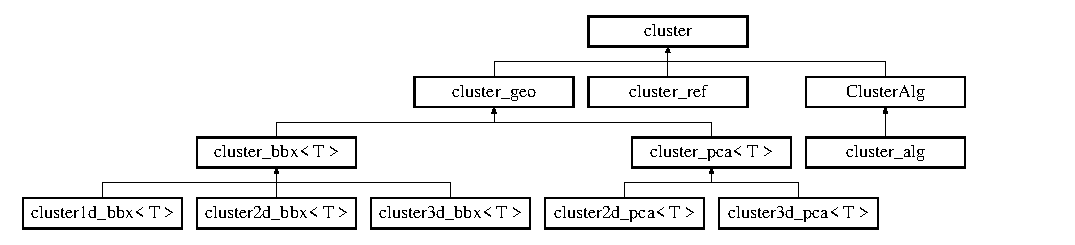
\includegraphics[height=2.849873cm]{classcluster}
\end{center}
\end{figure}
\subsection*{\-Public \-Member \-Functions}
\begin{DoxyCompactItemize}
\item 
\hyperlink{classcluster_a32fd64e14f672a22f4ee58fe856f1626}{cluster} (unsigned k, unsigned l)
\begin{DoxyCompactList}\small\item\em \-Constructor. \end{DoxyCompactList}\item 
virtual bool \hyperlink{classcluster_aa48a0f4aada61485263d76b82e819b4b}{isadm} (double eta2, \hyperlink{classcluster}{cluster} $\ast$cl, bl\-\_\-info \&info)=0
\item 
virtual void \hyperlink{classcluster_a7eb7a1209c0030e5cf344252f704fd57}{create\-Cluster\-Tree} (unsigned bmin, unsigned $\ast$op\-\_\-perm, unsigned $\ast$po\-\_\-perm)=0
\end{DoxyCompactItemize}
\subsection*{\-Protected \-Attributes}
\begin{DoxyCompactItemize}
\item 
\hypertarget{classcluster_ab4f61cd101a28c78d62deba9ebcd1a88}{
unsigned \hyperlink{classcluster_ab4f61cd101a28c78d62deba9ebcd1a88}{nbeg}}
\label{classcluster_ab4f61cd101a28c78d62deba9ebcd1a88}

\begin{DoxyCompactList}\small\item\em beginning and ending index (beginning index of next) \end{DoxyCompactList}\item 
\hypertarget{classcluster_a5351798cb6e92485a7e1b87d9b566546}{
unsigned \hyperlink{classcluster_a5351798cb6e92485a7e1b87d9b566546}{nsons}}
\label{classcluster_a5351798cb6e92485a7e1b87d9b566546}

\begin{DoxyCompactList}\small\item\em number of sons, nsons==0 if this is a leaf \end{DoxyCompactList}\item 
\hypertarget{classcluster_a8dae9741438a6597431995db720908db}{
\hyperlink{classcluster}{cluster} $\ast$$\ast$ \hyperlink{classcluster_a8dae9741438a6597431995db720908db}{sons}}
\label{classcluster_a8dae9741438a6597431995db720908db}

\begin{DoxyCompactList}\small\item\em the array of sons of this cluster in the cluster tree \end{DoxyCompactList}\end{DoxyCompactItemize}


\subsection{\-Detailed \-Description}
the basis class for storing clusters of degrees of freedom 

\subsection{\-Constructor \& \-Destructor \-Documentation}
\hypertarget{classcluster_a32fd64e14f672a22f4ee58fe856f1626}{
\index{cluster@{cluster}!cluster@{cluster}}
\index{cluster@{cluster}!cluster@{cluster}}
\subsubsection[{cluster}]{\setlength{\rightskip}{0pt plus 5cm}cluster\-::cluster (
\begin{DoxyParamCaption}
\item[{unsigned}]{k, }
\item[{unsigned}]{l}
\end{DoxyParamCaption}
)\hspace{0.3cm}{\ttfamily  \mbox{[}inline\mbox{]}}}}
\label{classcluster_a32fd64e14f672a22f4ee58fe856f1626}


\-Constructor. 


\begin{DoxyParams}{\-Parameters}
{\em k} & beginning index of the cluster \\
\hline
{\em l} & beginning index of the next cluster \\
\hline
\end{DoxyParams}


\subsection{\-Member \-Function \-Documentation}
\hypertarget{classcluster_a7eb7a1209c0030e5cf344252f704fd57}{
\index{cluster@{cluster}!create\-Cluster\-Tree@{create\-Cluster\-Tree}}
\index{create\-Cluster\-Tree@{create\-Cluster\-Tree}!cluster@{cluster}}
\subsubsection[{create\-Cluster\-Tree}]{\setlength{\rightskip}{0pt plus 5cm}virtual void cluster\-::create\-Cluster\-Tree (
\begin{DoxyParamCaption}
\item[{unsigned}]{bmin, }
\item[{unsigned $\ast$}]{op\-\_\-perm, }
\item[{unsigned $\ast$}]{po\-\_\-perm}
\end{DoxyParamCaption}
)\hspace{0.3cm}{\ttfamily  \mbox{[}pure virtual\mbox{]}}}}
\label{classcluster_a7eb7a1209c0030e5cf344252f704fd57}
creates recursively the cluster tree, i.\-e. changes the permutation op\-\_\-perm and po\-\_\-perm and create child cluster trees 
\begin{DoxyParams}{\-Parameters}
{\em op\-\_\-perm} & permutation\-: permutated\-\_\-row = op\-\_\-perm\mbox{[}original\-\_\-row\mbox{]} \\
\hline
{\em po\-\_\-perm} & reverse permutation\-: original\-\_\-row = po\-\_\-perm\mbox{[}permutated\-\_\-idx\mbox{]} \\
\hline
{\em bmin} & threshold value for stopping further refinement \\
\hline
\end{DoxyParams}


\-Implemented in \hyperlink{classcluster__pca_a269105a7c9520bdcc566a858fbf6b763}{cluster\-\_\-pca$<$ T $>$}, \hyperlink{classcluster__pca_a269105a7c9520bdcc566a858fbf6b763}{cluster\-\_\-pca$<$ T1 $>$}, \hyperlink{classcluster__pca_a269105a7c9520bdcc566a858fbf6b763}{cluster\-\_\-pca$<$ T2 $>$}, \hyperlink{classClusterAlg_acbbefef10e2d91713a567af5bb5c08f7}{\-Cluster\-Alg}, \hyperlink{classcluster__bbx_afa9ff45f3792189e25a46b8764f2da0c}{cluster\-\_\-bbx$<$ T $>$}, and \hyperlink{classcluster__alg_a2464aa83e8604d2098870c461f93b013}{cluster\-\_\-alg}.



\-Referenced by cluster\-\_\-bbx$<$ T $>$\-::create\-Cluster\-Tree(), and cluster\-\_\-pca$<$ T2 $>$\-::create\-Cluster\-Tree().

\hypertarget{classcluster_aa48a0f4aada61485263d76b82e819b4b}{
\index{cluster@{cluster}!isadm@{isadm}}
\index{isadm@{isadm}!cluster@{cluster}}
\subsubsection[{isadm}]{\setlength{\rightskip}{0pt plus 5cm}virtual bool cluster\-::isadm (
\begin{DoxyParamCaption}
\item[{double}]{eta2, }
\item[{{\bf cluster} $\ast$}]{cl, }
\item[{bl\-\_\-info \&}]{info}
\end{DoxyParamCaption}
)\hspace{0.3cm}{\ttfamily  \mbox{[}pure virtual\mbox{]}}}}
\label{classcluster_aa48a0f4aada61485263d76b82e819b4b}
is this cluster admissible with the cluster cl ? bool\& only valid for cluster\-Sp\-N\-D 

\-Implemented in \hyperlink{classcluster3d__bbx_a435d59e2b633d01a2748b7353168796e}{cluster3d\-\_\-bbx$<$ T $>$}, \hyperlink{classcluster2d__bbx_a0c0e1d9841ed93b2a59b241fc68135e6}{cluster2d\-\_\-bbx$<$ T $>$}, \hyperlink{classClusterAlg_a3daa14e294fe03b1405d057de3a640be}{\-Cluster\-Alg}, \hyperlink{classcluster1d__bbx_afbdd020333c05115e04969bef28db2cf}{cluster1d\-\_\-bbx$<$ T $>$}, \hyperlink{classcluster__alg_ae3c32452aca9733c237f0c23dc8f95e6}{cluster\-\_\-alg}, \hyperlink{classcluster__pca_a4546575a6d4e83e4d8ab6131019fae95}{cluster\-\_\-pca$<$ T $>$}, \hyperlink{classcluster__pca_a4546575a6d4e83e4d8ab6131019fae95}{cluster\-\_\-pca$<$ T1 $>$}, \hyperlink{classcluster__pca_a4546575a6d4e83e4d8ab6131019fae95}{cluster\-\_\-pca$<$ T2 $>$}, and \hyperlink{classcluster__bbx_ab5852c7c8fb33c1b3a681c8f4b0eec10}{cluster\-\_\-bbx$<$ T $>$}.



\-The documentation for this class was generated from the following file\-:\begin{DoxyCompactItemize}
\item 
\hyperlink{cluster_8h}{cluster.\-h}\end{DoxyCompactItemize}

\hypertarget{classcluster1d__bbx}{
\section{cluster1d\-\_\-bbx$<$ \-T $>$ \-Class \-Template \-Reference}
\label{classcluster1d__bbx}\index{cluster1d\-\_\-bbx$<$ T $>$@{cluster1d\-\_\-bbx$<$ T $>$}}
}


a class for storing clusters of degrees of freedom in 1d  




{\ttfamily \#include $<$cluster\-\_\-bbx.\-h$>$}

\-Inheritance diagram for cluster1d\-\_\-bbx$<$ \-T $>$\-:\begin{figure}[H]
\begin{center}
\leavevmode
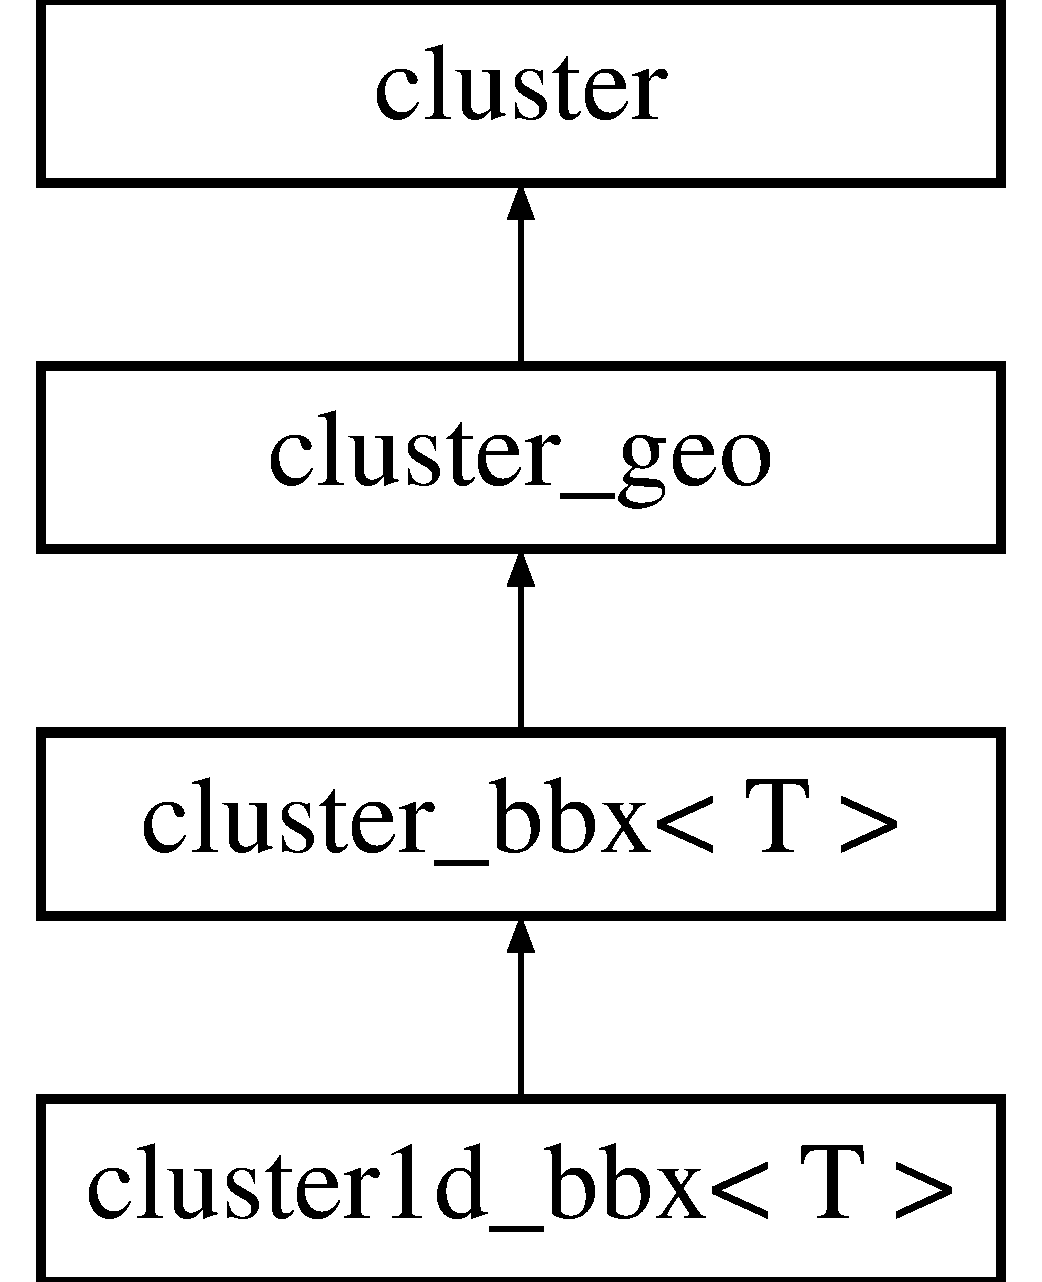
\includegraphics[height=4.000000cm]{classcluster1d__bbx}
\end{center}
\end{figure}
\subsection*{\-Public \-Member \-Functions}
\begin{DoxyCompactItemize}
\item 
bool \hyperlink{classcluster1d__bbx_afbdd020333c05115e04969bef28db2cf}{isadm} (double eta, \hyperlink{classcluster}{cluster} $\ast$cl, bl\-\_\-info \&info)
\end{DoxyCompactItemize}
\subsection*{\-Protected \-Member \-Functions}
\begin{DoxyCompactItemize}
\item 
\hypertarget{classcluster1d__bbx_a897f33d1e275ac795bda3ed5447bd530}{
virtual unsigned \hyperlink{classcluster1d__bbx_a897f33d1e275ac795bda3ed5447bd530}{dim} () const }
\label{classcluster1d__bbx_a897f33d1e275ac795bda3ed5447bd530}

\begin{DoxyCompactList}\small\item\em returns the spatial dimension \end{DoxyCompactList}\end{DoxyCompactItemize}


\subsection{\-Detailed \-Description}
\subsubsection*{template$<$class \-T$>$class cluster1d\-\_\-bbx$<$ T $>$}

a class for storing clusters of degrees of freedom in 1d 

\subsection{\-Member \-Function \-Documentation}
\hypertarget{classcluster1d__bbx_afbdd020333c05115e04969bef28db2cf}{
\index{cluster1d\-\_\-bbx@{cluster1d\-\_\-bbx}!isadm@{isadm}}
\index{isadm@{isadm}!cluster1d_bbx@{cluster1d\-\_\-bbx}}
\subsubsection[{isadm}]{\setlength{\rightskip}{0pt plus 5cm}template$<$class \-T$>$ bool {\bf cluster1d\-\_\-bbx}$<$ \-T $>$\-::isadm (
\begin{DoxyParamCaption}
\item[{double}]{eta2, }
\item[{{\bf cluster} $\ast$}]{cl, }
\item[{bl\-\_\-info \&}]{info}
\end{DoxyParamCaption}
)\hspace{0.3cm}{\ttfamily  \mbox{[}inline, virtual\mbox{]}}}}
\label{classcluster1d__bbx_afbdd020333c05115e04969bef28db2cf}
is this cluster admissible with the cluster cl ? bool\& only valid for cluster\-Sp\-N\-D 

\-Implements \hyperlink{classcluster__bbx_ab5852c7c8fb33c1b3a681c8f4b0eec10}{cluster\-\_\-bbx$<$ T $>$}.



\-References cluster\-\_\-geo\-::diam2.



\-The documentation for this class was generated from the following file\-:\begin{DoxyCompactItemize}
\item 
cluster\-\_\-bbx.\-h\end{DoxyCompactItemize}

\hypertarget{classcluster2d__bbx}{
\section{cluster2d\-\_\-bbx$<$ \-T $>$ \-Class \-Template \-Reference}
\label{classcluster2d__bbx}\index{cluster2d\-\_\-bbx$<$ T $>$@{cluster2d\-\_\-bbx$<$ T $>$}}
}


a class for storing clusters of degrees of freedom in 2d  




{\ttfamily \#include $<$cluster\-\_\-bbx.\-h$>$}

\-Inheritance diagram for cluster2d\-\_\-bbx$<$ \-T $>$\-:\begin{figure}[H]
\begin{center}
\leavevmode
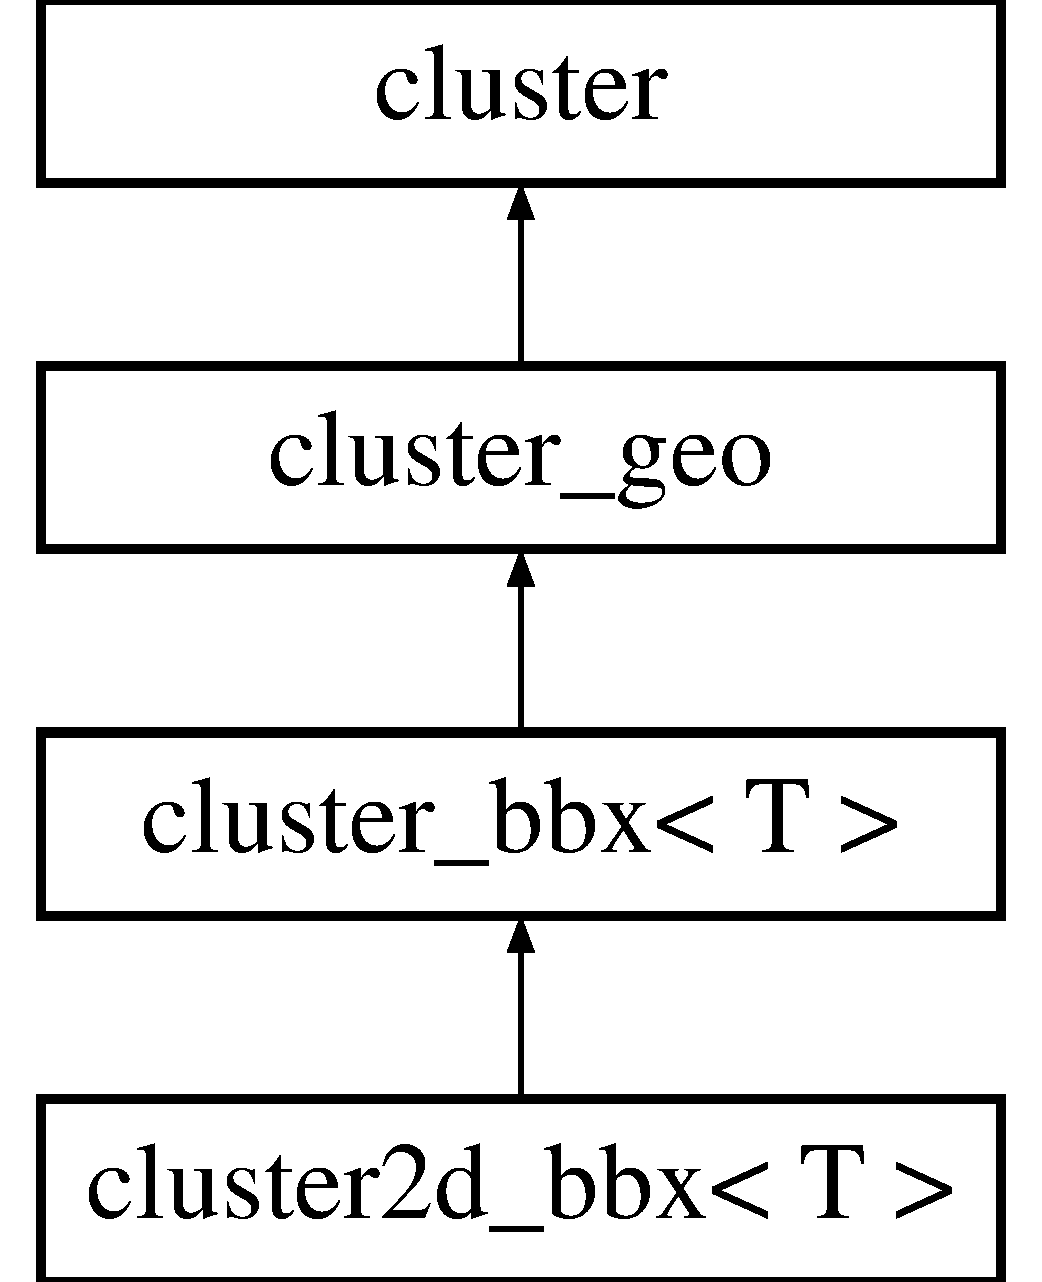
\includegraphics[height=4.000000cm]{classcluster2d__bbx}
\end{center}
\end{figure}
\subsection*{\-Public \-Member \-Functions}
\begin{DoxyCompactItemize}
\item 
bool \hyperlink{classcluster2d__bbx_a0c0e1d9841ed93b2a59b241fc68135e6}{isadm} (double eta, \hyperlink{classcluster}{cluster} $\ast$cl, bl\-\_\-info \&info)
\end{DoxyCompactItemize}
\subsection*{\-Protected \-Member \-Functions}
\begin{DoxyCompactItemize}
\item 
\hypertarget{classcluster2d__bbx_a1f4b5d08dcf3517cdb6e4c4f356a9495}{
virtual unsigned \hyperlink{classcluster2d__bbx_a1f4b5d08dcf3517cdb6e4c4f356a9495}{dim} () const }
\label{classcluster2d__bbx_a1f4b5d08dcf3517cdb6e4c4f356a9495}

\begin{DoxyCompactList}\small\item\em returns the spatial dimension \end{DoxyCompactList}\end{DoxyCompactItemize}


\subsection{\-Detailed \-Description}
\subsubsection*{template$<$class \-T$>$class cluster2d\-\_\-bbx$<$ T $>$}

a class for storing clusters of degrees of freedom in 2d 

\subsection{\-Member \-Function \-Documentation}
\hypertarget{classcluster2d__bbx_a0c0e1d9841ed93b2a59b241fc68135e6}{
\index{cluster2d\-\_\-bbx@{cluster2d\-\_\-bbx}!isadm@{isadm}}
\index{isadm@{isadm}!cluster2d_bbx@{cluster2d\-\_\-bbx}}
\subsubsection[{isadm}]{\setlength{\rightskip}{0pt plus 5cm}template$<$class \-T$>$ bool {\bf cluster2d\-\_\-bbx}$<$ \-T $>$\-::isadm (
\begin{DoxyParamCaption}
\item[{double}]{eta2, }
\item[{{\bf cluster} $\ast$}]{cl, }
\item[{bl\-\_\-info \&}]{info}
\end{DoxyParamCaption}
)\hspace{0.3cm}{\ttfamily  \mbox{[}inline, virtual\mbox{]}}}}
\label{classcluster2d__bbx_a0c0e1d9841ed93b2a59b241fc68135e6}
is this cluster admissible with the cluster cl ? bool\& only valid for cluster\-Sp\-N\-D 

\-Implements \hyperlink{classcluster__bbx_ab5852c7c8fb33c1b3a681c8f4b0eec10}{cluster\-\_\-bbx$<$ T $>$}.



\-References cluster\-\_\-geo\-::diam2.



\-The documentation for this class was generated from the following file\-:\begin{DoxyCompactItemize}
\item 
cluster\-\_\-bbx.\-h\end{DoxyCompactItemize}

\hypertarget{classcluster2d__pca}{
\section{cluster2d\-\_\-pca$<$ \-T $>$ \-Class \-Template \-Reference}
\label{classcluster2d__pca}\index{cluster2d\-\_\-pca$<$ T $>$@{cluster2d\-\_\-pca$<$ T $>$}}
}


a class for storing clusters of degrees of freedom in 2d  




{\ttfamily \#include $<$cluster\-\_\-pca.\-h$>$}

\-Inheritance diagram for cluster2d\-\_\-pca$<$ \-T $>$\-:\begin{figure}[H]
\begin{center}
\leavevmode
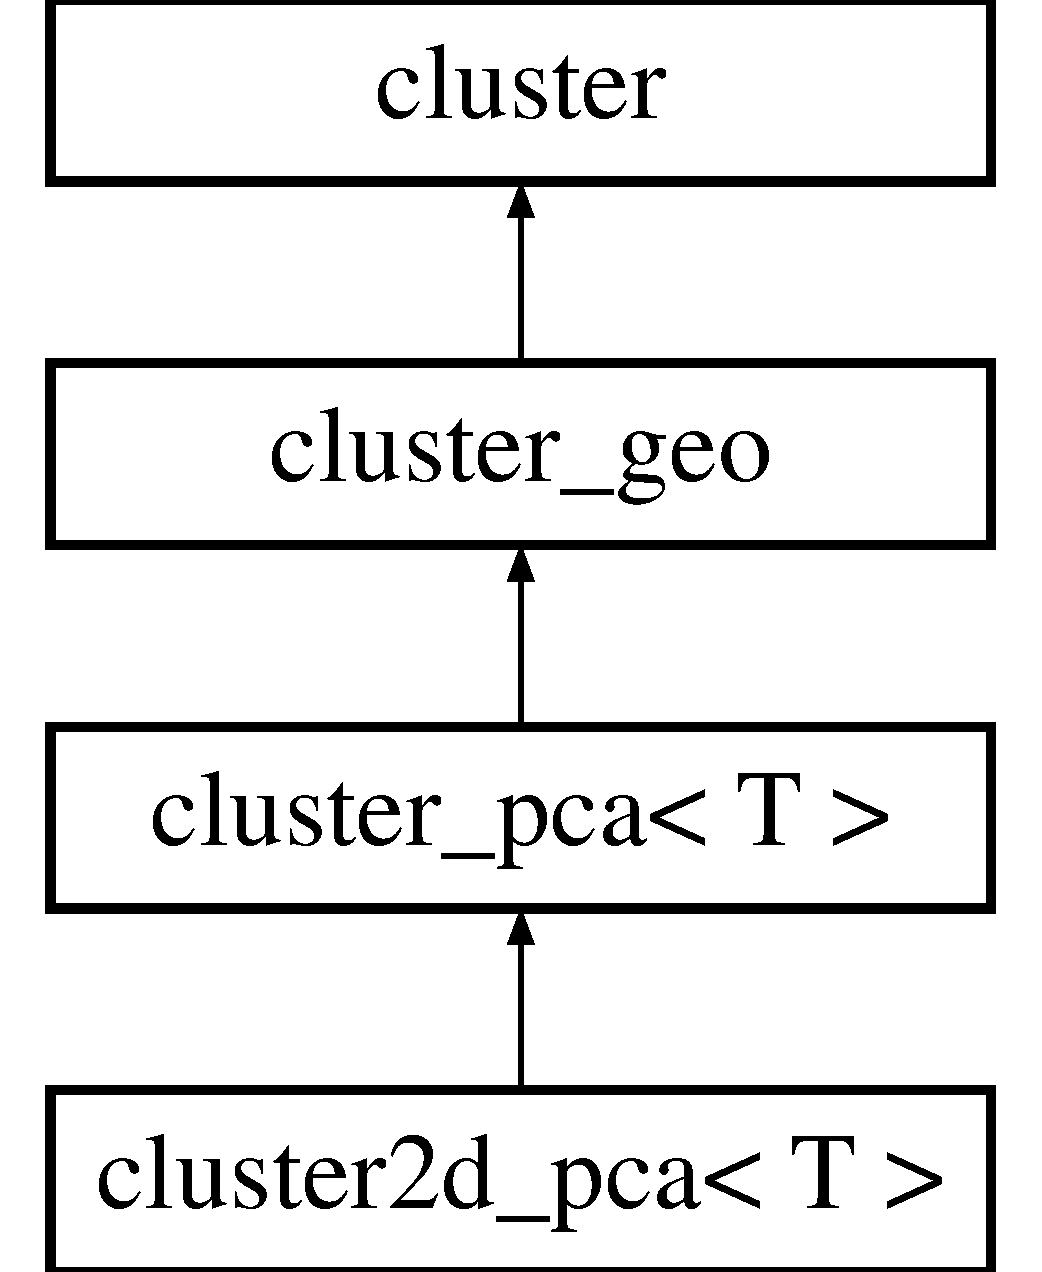
\includegraphics[height=4.000000cm]{classcluster2d__pca}
\end{center}
\end{figure}
\subsection*{\-Protected \-Member \-Functions}
\begin{DoxyCompactItemize}
\item 
\hypertarget{classcluster2d__pca_a70cb3c2ad43e60f7ff7908f8d063f99b}{
virtual unsigned \hyperlink{classcluster2d__pca_a70cb3c2ad43e60f7ff7908f8d063f99b}{dim} () const }
\label{classcluster2d__pca_a70cb3c2ad43e60f7ff7908f8d063f99b}

\begin{DoxyCompactList}\small\item\em returns the spatial dimension \end{DoxyCompactList}\end{DoxyCompactItemize}


\subsection{\-Detailed \-Description}
\subsubsection*{template$<$class \-T$>$class cluster2d\-\_\-pca$<$ T $>$}

a class for storing clusters of degrees of freedom in 2d 

\-The documentation for this class was generated from the following file\-:\begin{DoxyCompactItemize}
\item 
\hyperlink{cluster__pca_8h}{cluster\-\_\-pca.\-h}\end{DoxyCompactItemize}

\hypertarget{classcluster3d__bbx}{
\section{cluster3d\-\_\-bbx$<$ \-T $>$ \-Class \-Template \-Reference}
\label{classcluster3d__bbx}\index{cluster3d\-\_\-bbx$<$ T $>$@{cluster3d\-\_\-bbx$<$ T $>$}}
}


a class for storing clusters of degrees of freedom in 3d  




{\ttfamily \#include $<$cluster\-\_\-bbx.\-h$>$}

\-Inheritance diagram for cluster3d\-\_\-bbx$<$ \-T $>$\-:\begin{figure}[H]
\begin{center}
\leavevmode
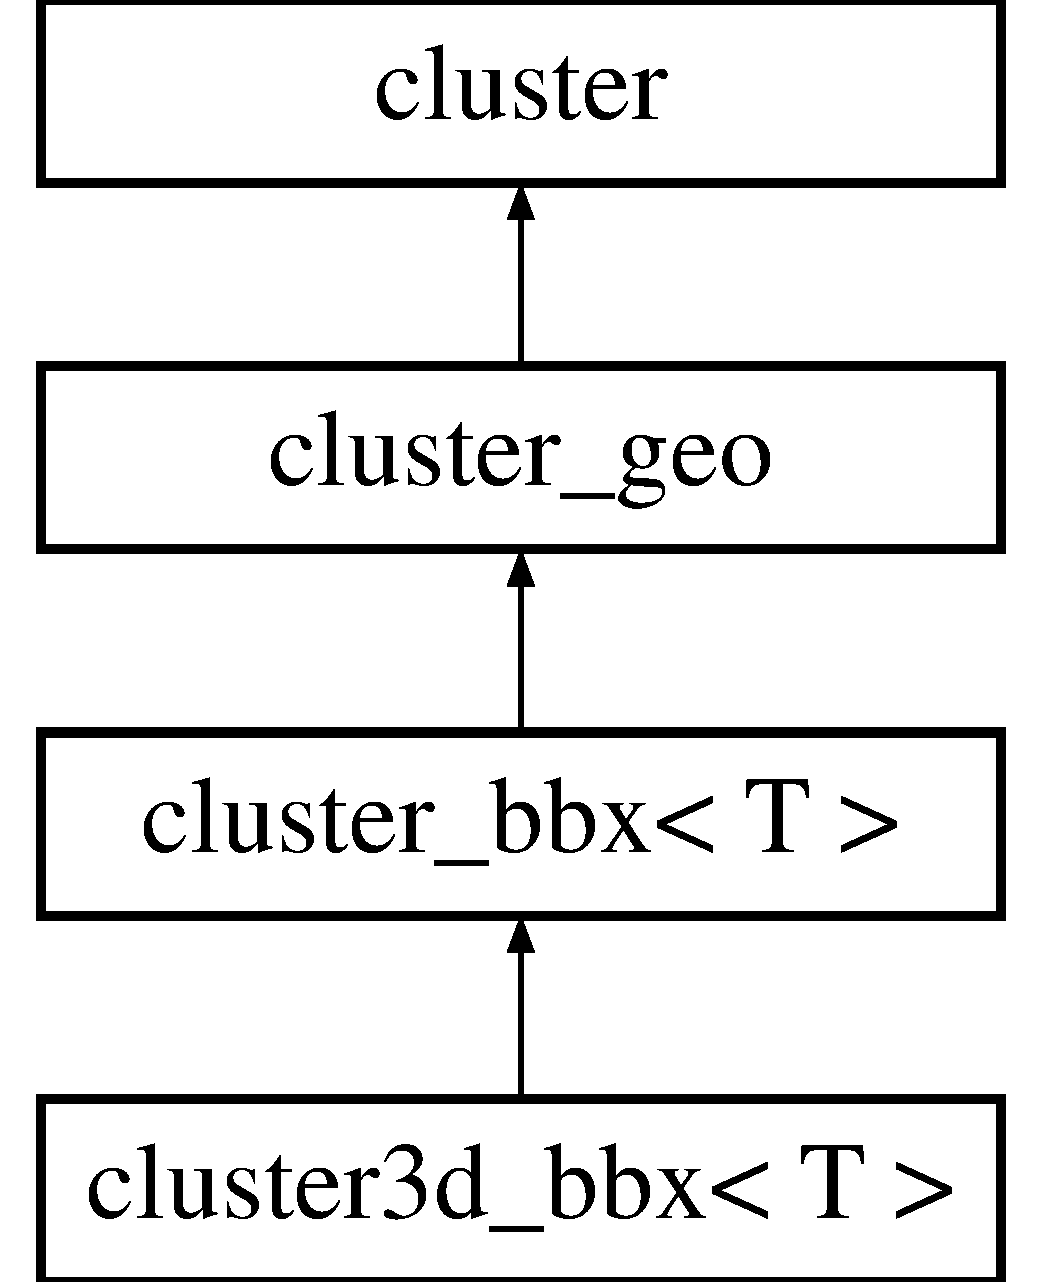
\includegraphics[height=4.000000cm]{classcluster3d__bbx}
\end{center}
\end{figure}
\subsection*{\-Public \-Member \-Functions}
\begin{DoxyCompactItemize}
\item 
bool \hyperlink{classcluster3d__bbx_a435d59e2b633d01a2748b7353168796e}{isadm} (double eta, \hyperlink{classcluster}{cluster} $\ast$cl, bl\-\_\-info \&info)
\end{DoxyCompactItemize}
\subsection*{\-Protected \-Member \-Functions}
\begin{DoxyCompactItemize}
\item 
\hypertarget{classcluster3d__bbx_a249df479ab36acd3151163eae90098dc}{
virtual unsigned \hyperlink{classcluster3d__bbx_a249df479ab36acd3151163eae90098dc}{dim} () const }
\label{classcluster3d__bbx_a249df479ab36acd3151163eae90098dc}

\begin{DoxyCompactList}\small\item\em returns the spatial dimension \end{DoxyCompactList}\end{DoxyCompactItemize}


\subsection{\-Detailed \-Description}
\subsubsection*{template$<$class \-T$>$class cluster3d\-\_\-bbx$<$ T $>$}

a class for storing clusters of degrees of freedom in 3d 

\subsection{\-Member \-Function \-Documentation}
\hypertarget{classcluster3d__bbx_a435d59e2b633d01a2748b7353168796e}{
\index{cluster3d\-\_\-bbx@{cluster3d\-\_\-bbx}!isadm@{isadm}}
\index{isadm@{isadm}!cluster3d_bbx@{cluster3d\-\_\-bbx}}
\subsubsection[{isadm}]{\setlength{\rightskip}{0pt plus 5cm}template$<$class \-T$>$ bool {\bf cluster3d\-\_\-bbx}$<$ \-T $>$\-::isadm (
\begin{DoxyParamCaption}
\item[{double}]{eta2, }
\item[{{\bf cluster} $\ast$}]{cl, }
\item[{bl\-\_\-info \&}]{info}
\end{DoxyParamCaption}
)\hspace{0.3cm}{\ttfamily  \mbox{[}inline, virtual\mbox{]}}}}
\label{classcluster3d__bbx_a435d59e2b633d01a2748b7353168796e}
is this cluster admissible with the cluster cl ? bool\& only valid for cluster\-Sp\-N\-D 

\-Implements \hyperlink{classcluster__bbx_ab5852c7c8fb33c1b3a681c8f4b0eec10}{cluster\-\_\-bbx$<$ T $>$}.



\-References cluster\-\_\-geo\-::diam2.



\-The documentation for this class was generated from the following file\-:\begin{DoxyCompactItemize}
\item 
cluster\-\_\-bbx.\-h\end{DoxyCompactItemize}

\hypertarget{classcluster3d__pca}{
\section{cluster3d\-\_\-pca$<$ \-T $>$ \-Class \-Template \-Reference}
\label{classcluster3d__pca}\index{cluster3d\-\_\-pca$<$ T $>$@{cluster3d\-\_\-pca$<$ T $>$}}
}


a class for storing clusters of degrees of freedom in 3d  




{\ttfamily \#include $<$cluster\-\_\-pca.\-h$>$}

\-Inheritance diagram for cluster3d\-\_\-pca$<$ \-T $>$\-:\begin{figure}[H]
\begin{center}
\leavevmode
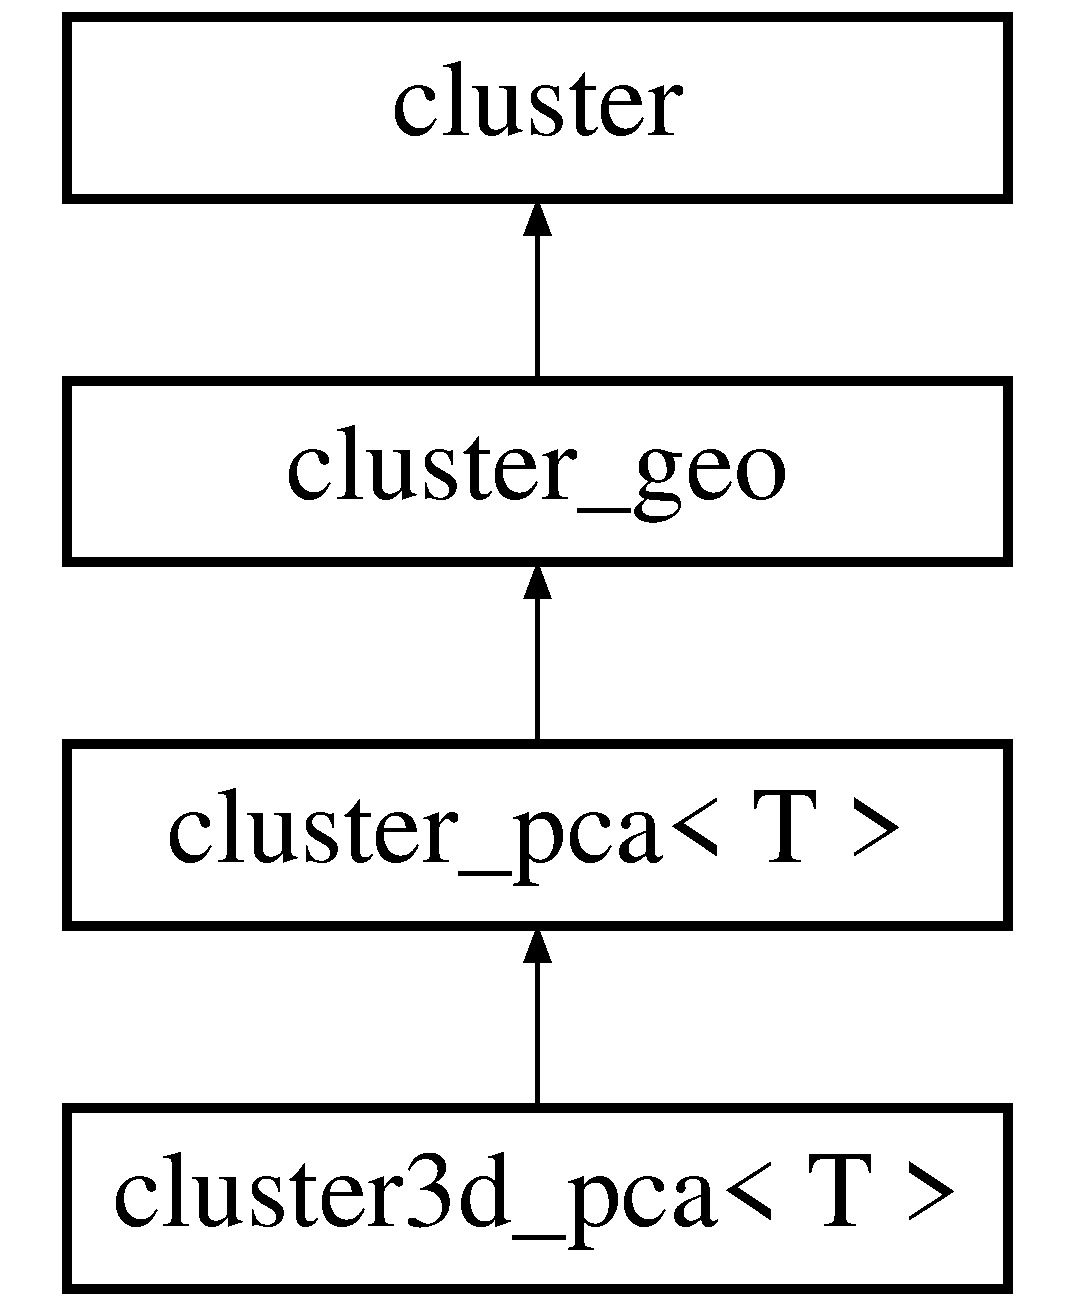
\includegraphics[height=4.000000cm]{classcluster3d__pca}
\end{center}
\end{figure}
\subsection*{\-Protected \-Member \-Functions}
\begin{DoxyCompactItemize}
\item 
\hypertarget{classcluster3d__pca_ad8e00a2e23452c2f4a52c815e5110770}{
virtual unsigned \hyperlink{classcluster3d__pca_ad8e00a2e23452c2f4a52c815e5110770}{dim} () const }
\label{classcluster3d__pca_ad8e00a2e23452c2f4a52c815e5110770}

\begin{DoxyCompactList}\small\item\em returns the spatial dimension \end{DoxyCompactList}\end{DoxyCompactItemize}


\subsection{\-Detailed \-Description}
\subsubsection*{template$<$class \-T$>$class cluster3d\-\_\-pca$<$ T $>$}

a class for storing clusters of degrees of freedom in 3d 

\-The documentation for this class was generated from the following file\-:\begin{DoxyCompactItemize}
\item 
\hyperlink{cluster__pca_8h}{cluster\-\_\-pca.\-h}\end{DoxyCompactItemize}

\hypertarget{classcluster__alg}{
\section{cluster\-\_\-alg \-Class \-Reference}
\label{classcluster__alg}\index{cluster\-\_\-alg@{cluster\-\_\-alg}}
}


class for storing clusters of degrees of freedom without geometric information. \-This class stores clusters (no separators)  




{\ttfamily \#include $<$cluster\-\_\-alg.\-h$>$}

\-Inheritance diagram for cluster\-\_\-alg\-:\begin{figure}[H]
\begin{center}
\leavevmode
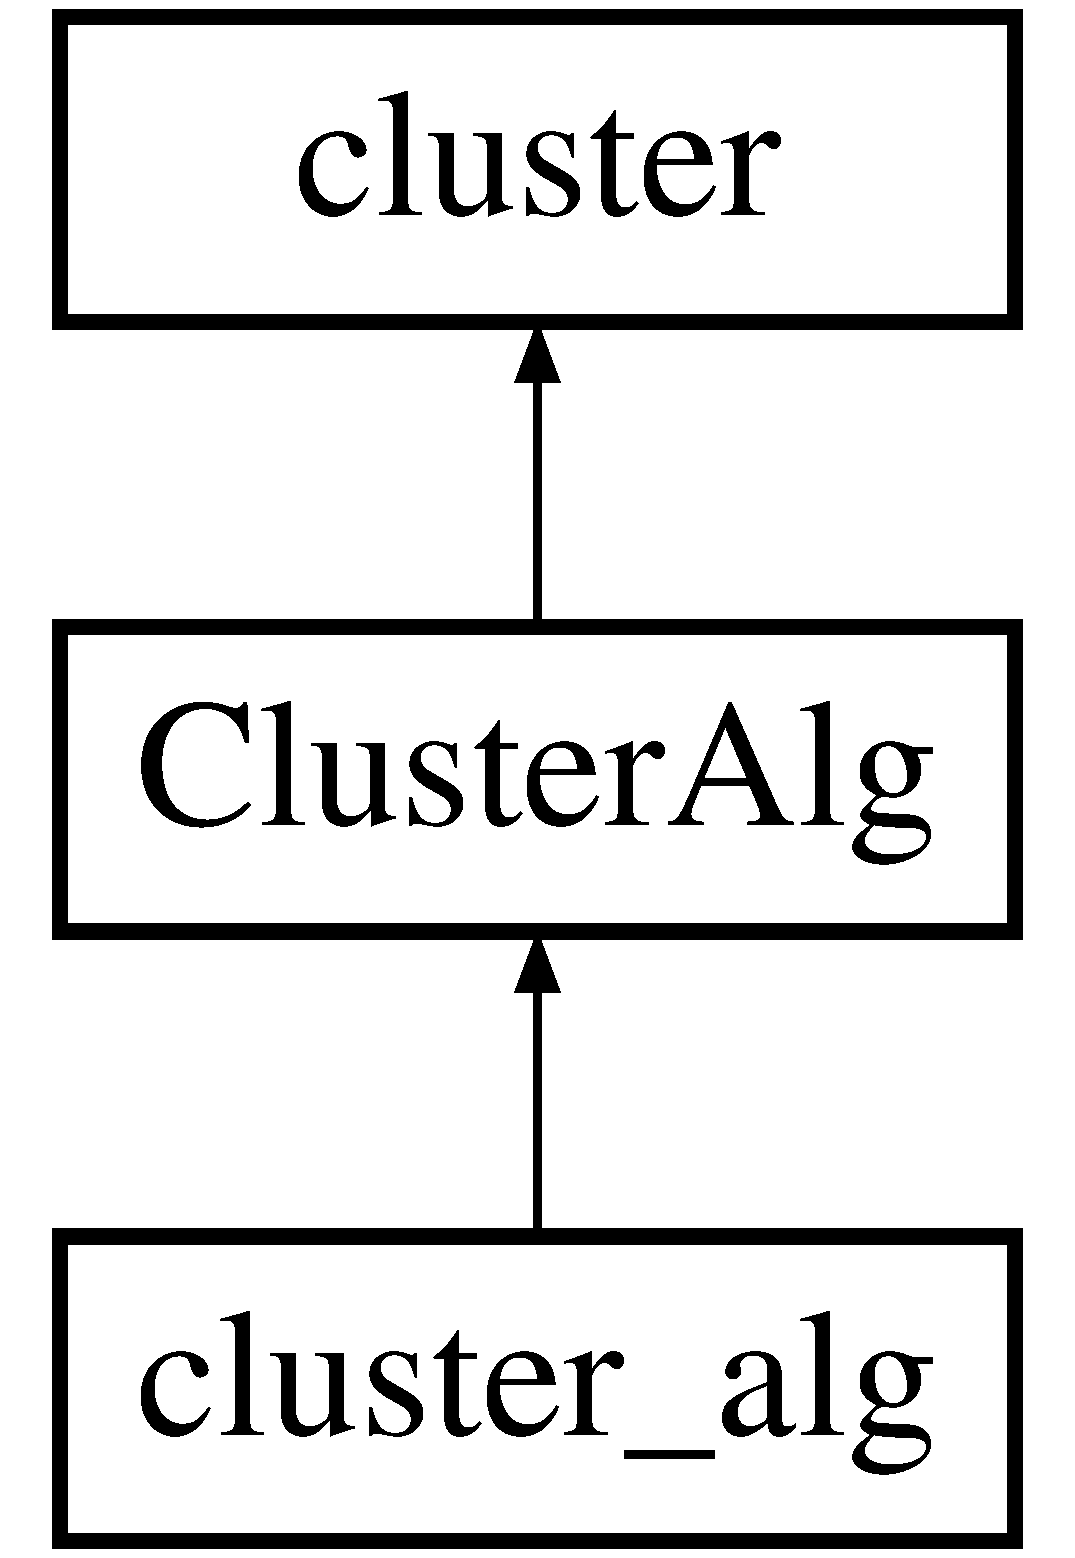
\includegraphics[height=3.000000cm]{classcluster__alg}
\end{center}
\end{figure}
\subsection*{\-Public \-Member \-Functions}
\begin{DoxyCompactItemize}
\item 
\hyperlink{classcluster__alg_a7b80a55ab14ddfd8a6c9f67953768240}{cluster\-\_\-alg} (unsigned n, unsigned $\ast$i\-A, unsigned $\ast$j\-A)
\item 
virtual \hyperlink{classcluster__alg_a2f0e2dfe7df931fc2a7161e19b77622b}{$\sim$cluster\-\_\-alg} ()
\item 
virtual void \hyperlink{classcluster__alg_a2464aa83e8604d2098870c461f93b013}{create\-Cluster\-Tree} (unsigned bmin, unsigned $\ast$\hyperlink{classClusterAlg_a4f06e1465978072d8c6bd098e062b701}{op\-\_\-perm}, unsigned $\ast$\hyperlink{classClusterAlg_af3d1d7c4ae0516ff9de725d3ff760b07}{po\-\_\-perm})
\item 
bool \hyperlink{classcluster__alg_ae3c32452aca9733c237f0c23dc8f95e6}{isadm} (double eta2, \hyperlink{classcluster}{cluster} $\ast$cl, bl\-\_\-info \&info)
\begin{DoxyCompactList}\small\item\em \-This method checks the admissibility of the cluster represented by this object and the cluster cl given as parameter to isadm. \end{DoxyCompactList}\item 
virtual bool \hyperlink{classcluster__alg_a20b9fac849beaf8b760e3bb15fae66e0}{is\-Separator} () const 
\end{DoxyCompactItemize}
\subsection*{\-Protected \-Member \-Functions}
\begin{DoxyCompactItemize}
\item 
\hyperlink{classcluster__alg_ae9955a23c000cde86b67d662c06912f1}{cluster\-\_\-alg} (\hyperlink{classClusterAlg}{\-Cluster\-Alg} $\ast$father, unsigned beg, unsigned end, unsigned $\ast$\hyperlink{classClusterAlg_a4f06e1465978072d8c6bd098e062b701}{op\-\_\-perm}, unsigned $\ast$\hyperlink{classClusterAlg_af3d1d7c4ae0516ff9de725d3ff760b07}{po\-\_\-perm}, unsigned \hyperlink{classClusterAlg_ac06ccb0ba85be10e97392bd063fa78c8}{depth}, \-Adj\-Mat $\ast$global\-\_\-mat, \-Adj\-Mat $\ast$local\-\_\-mat)
\begin{DoxyCompactList}\small\item\em \-Constructor. \end{DoxyCompactList}\item 
void \hyperlink{classcluster__alg_a289d2fce6fba6f3452468a99d6a81ff3}{update\-Perm} (unsigned $\ast$reordering, unsigned \&isep0, unsigned \&isep1)
\item 
virtual void \hyperlink{classcluster__alg_a78292c11a717fb5b83762fc4c070797f}{compute\-Neighbor} ()
\item 
void \hyperlink{classcluster__alg_a411de6be2059e0c2848c4b11f9a043cf}{subdivide} (unsigned bmin)
\begin{DoxyCompactList}\small\item\em subdivide this cluster recursively, needed to generate the cluster tree \end{DoxyCompactList}\end{DoxyCompactItemize}


\subsection{\-Detailed \-Description}
class for storing clusters of degrees of freedom without geometric information. \-This class stores clusters (no separators) 

\subsection{\-Constructor \& \-Destructor \-Documentation}
\hypertarget{classcluster__alg_a7b80a55ab14ddfd8a6c9f67953768240}{
\index{cluster\-\_\-alg@{cluster\-\_\-alg}!cluster\-\_\-alg@{cluster\-\_\-alg}}
\index{cluster\-\_\-alg@{cluster\-\_\-alg}!cluster_alg@{cluster\-\_\-alg}}
\subsubsection[{cluster\-\_\-alg}]{\setlength{\rightskip}{0pt plus 5cm}cluster\-\_\-alg\-::cluster\-\_\-alg (
\begin{DoxyParamCaption}
\item[{unsigned}]{n, }
\item[{unsigned $\ast$}]{i\-A, }
\item[{unsigned $\ast$}]{j\-A}
\end{DoxyParamCaption}
)\hspace{0.3cm}{\ttfamily  \mbox{[}inline\mbox{]}}}}
\label{classcluster__alg_a7b80a55ab14ddfd8a6c9f67953768240}
\-Constructor creates the root of the cluster tree 
\begin{DoxyParams}{\-Parameters}
{\em n} & \\
\hline
{\em j\-A} & \\
\hline
{\em i\-A} & \\
\hline
\end{DoxyParams}
\begin{DoxyReturn}{\-Returns}

\end{DoxyReturn}
\hypertarget{classcluster__alg_ae9955a23c000cde86b67d662c06912f1}{
\index{cluster\-\_\-alg@{cluster\-\_\-alg}!cluster\-\_\-alg@{cluster\-\_\-alg}}
\index{cluster\-\_\-alg@{cluster\-\_\-alg}!cluster_alg@{cluster\-\_\-alg}}
\subsubsection[{cluster\-\_\-alg}]{\setlength{\rightskip}{0pt plus 5cm}cluster\-\_\-alg\-::cluster\-\_\-alg (
\begin{DoxyParamCaption}
\item[{{\bf \-Cluster\-Alg} $\ast$}]{father, }
\item[{unsigned}]{beg, }
\item[{unsigned}]{end, }
\item[{unsigned $\ast$}]{op\-\_\-perm, }
\item[{unsigned $\ast$}]{po\-\_\-perm, }
\item[{unsigned}]{depth, }
\item[{\-Adj\-Mat $\ast$}]{global\-\_\-mat, }
\item[{\-Adj\-Mat $\ast$}]{local\-\_\-mat}
\end{DoxyParamCaption}
)\hspace{0.3cm}{\ttfamily  \mbox{[}inline, protected\mbox{]}}}}
\label{classcluster__alg_ae9955a23c000cde86b67d662c06912f1}


\-Constructor. 


\begin{DoxyParams}{\-Parameters}
{\em father} & parent node in cluster tree \\
\hline
{\em beg} & beginning index of the cluster \\
\hline
{\em end} & beginning index of the next cluster \\
\hline
{\em op\-\_\-perm} & permutation \\
\hline
{\em po\-\_\-perm} & permutation \\
\hline
{\em depth} & distance between this node and the root \\
\hline
{\em global\-\_\-mat} & reference to adjacency matrix of the matrix graph in crs format \\
\hline
{\em local\-\_\-mat} & pointer to the local adjacency matrix of the matrix graph in crs format \\
\hline
\end{DoxyParams}
\hypertarget{classcluster__alg_a2f0e2dfe7df931fc2a7161e19b77622b}{
\index{cluster\-\_\-alg@{cluster\-\_\-alg}!$\sim$cluster\-\_\-alg@{$\sim$cluster\-\_\-alg}}
\index{$\sim$cluster\-\_\-alg@{$\sim$cluster\-\_\-alg}!cluster_alg@{cluster\-\_\-alg}}
\subsubsection[{$\sim$cluster\-\_\-alg}]{\setlength{\rightskip}{0pt plus 5cm}virtual cluster\-\_\-alg\-::$\sim$cluster\-\_\-alg (
\begin{DoxyParamCaption}
{}
\end{DoxyParamCaption}
)\hspace{0.3cm}{\ttfamily  \mbox{[}inline, virtual\mbox{]}}}}
\label{classcluster__alg_a2f0e2dfe7df931fc2a7161e19b77622b}
\-Destructor. 

\subsection{\-Member \-Function \-Documentation}
\hypertarget{classcluster__alg_a78292c11a717fb5b83762fc4c070797f}{
\index{cluster\-\_\-alg@{cluster\-\_\-alg}!compute\-Neighbor@{compute\-Neighbor}}
\index{compute\-Neighbor@{compute\-Neighbor}!cluster_alg@{cluster\-\_\-alg}}
\subsubsection[{compute\-Neighbor}]{\setlength{\rightskip}{0pt plus 5cm}virtual void cluster\-\_\-alg\-::compute\-Neighbor (
\begin{DoxyParamCaption}
{}
\end{DoxyParamCaption}
)\hspace{0.3cm}{\ttfamily  \mbox{[}protected, virtual\mbox{]}}}}
\label{classcluster__alg_a78292c11a717fb5b83762fc4c070797f}
\-Method traverses the \hyperlink{classClusterAlg}{\-Cluster\-Alg} tree and computes the boundary clusters of the actual cluster that consists of the sibling-\/separator and parts of other separators from higher levels. 

\-Implements \hyperlink{classClusterAlg_a3da066d722da219e5f64f624a6121b05}{\-Cluster\-Alg}.

\hypertarget{classcluster__alg_a2464aa83e8604d2098870c461f93b013}{
\index{cluster\-\_\-alg@{cluster\-\_\-alg}!create\-Cluster\-Tree@{create\-Cluster\-Tree}}
\index{create\-Cluster\-Tree@{create\-Cluster\-Tree}!cluster_alg@{cluster\-\_\-alg}}
\subsubsection[{create\-Cluster\-Tree}]{\setlength{\rightskip}{0pt plus 5cm}virtual void cluster\-\_\-alg\-::create\-Cluster\-Tree (
\begin{DoxyParamCaption}
\item[{unsigned}]{bmin, }
\item[{unsigned $\ast$}]{op\-\_\-perm, }
\item[{unsigned $\ast$}]{po\-\_\-perm}
\end{DoxyParamCaption}
)\hspace{0.3cm}{\ttfamily  \mbox{[}virtual\mbox{]}}}}
\label{classcluster__alg_a2464aa83e8604d2098870c461f93b013}
\-Method creates recursively the cluster tree, i.\-e. changes the permutation op\-\_\-perm and po\-\_\-perm and create child cluster trees. \-For this task only the adjacency matrix is used. 
\begin{DoxyParams}{\-Parameters}
{\em op\-\_\-perm} & permutation\-: permutated\-\_\-row = op\-\_\-perm\mbox{[}original\-\_\-row\mbox{]} \\
\hline
{\em po\-\_\-perm} & reverse permutation\-: original\-\_\-row = po\-\_\-perm\mbox{[}permutated\-\_\-idx\mbox{]} \\
\hline
{\em bmin} & threshold value for stopping further refinement \\
\hline
\end{DoxyParams}
\begin{DoxyReturn}{\-Returns}
a cluster tree 
\end{DoxyReturn}


\-Reimplemented from \hyperlink{classClusterAlg_acbbefef10e2d91713a567af5bb5c08f7}{\-Cluster\-Alg}.

\hypertarget{classcluster__alg_ae3c32452aca9733c237f0c23dc8f95e6}{
\index{cluster\-\_\-alg@{cluster\-\_\-alg}!isadm@{isadm}}
\index{isadm@{isadm}!cluster_alg@{cluster\-\_\-alg}}
\subsubsection[{isadm}]{\setlength{\rightskip}{0pt plus 5cm}bool cluster\-\_\-alg\-::isadm (
\begin{DoxyParamCaption}
\item[{double}]{eta2, }
\item[{{\bf cluster} $\ast$}]{cl, }
\item[{bl\-\_\-info \&}]{info}
\end{DoxyParamCaption}
)\hspace{0.3cm}{\ttfamily  \mbox{[}virtual\mbox{]}}}}
\label{classcluster__alg_ae3c32452aca9733c237f0c23dc8f95e6}


\-This method checks the admissibility of the cluster represented by this object and the cluster cl given as parameter to isadm. 

\-If both clusters are not separators then isadm returns true and the parameter info.\-is\-\_\-adm is set true, too. (because of nested dissection reordering)

\-If cluster cl is a separator, then method isadm tests if cl belongs to the nearfield or farfield of the cluster represented by this object. \-First the neighbourhood is checked. \-If cl and this object are not in neighbourhood it is necesarry to compute the distance between them. \-Therefor isadm computes an approximation of the distance between the accordingly clusters/nodes in dual graph (see get\-Dist()) and an approximation of the diameter of the cluster (see \hyperlink{classClusterAlg_aa2c3643c9a48e40c8adb7acbd3011ec5}{get\-Diam()}).


\begin{DoxyParams}{\-Parameters}
{\em eta2} & parameter to justify the admissibility condition (input) \\
\hline
{\em cl} & check the admissibility for cluster this and cluster cl (input) \\
\hline
{\em info} & the two attributes info.\-is\-\_\-adm and info.\-is\-\_\-sep are set (output) \\
\hline
\end{DoxyParams}
\begin{DoxyReturn}{\-Returns}
true if the clusters are admissible else false 
\end{DoxyReturn}


\-Implements \hyperlink{classClusterAlg_a3daa14e294fe03b1405d057de3a640be}{\-Cluster\-Alg}.

\hypertarget{classcluster__alg_a20b9fac849beaf8b760e3bb15fae66e0}{
\index{cluster\-\_\-alg@{cluster\-\_\-alg}!is\-Separator@{is\-Separator}}
\index{is\-Separator@{is\-Separator}!cluster_alg@{cluster\-\_\-alg}}
\subsubsection[{is\-Separator}]{\setlength{\rightskip}{0pt plus 5cm}virtual bool cluster\-\_\-alg\-::is\-Separator (
\begin{DoxyParamCaption}
{}
\end{DoxyParamCaption}
) const\hspace{0.3cm}{\ttfamily  \mbox{[}inline, virtual\mbox{]}}}}
\label{classcluster__alg_a20b9fac849beaf8b760e3bb15fae66e0}
\-Method returns the status of this \hyperlink{classClusterAlg}{\-Cluster\-Alg} object. \-Instances of this class are \char`\"{}normal\char`\"{} \-Clusters. \begin{DoxyReturn}{\-Returns}
false 
\end{DoxyReturn}


\-Implements \hyperlink{classClusterAlg_abe3332e66bad89111412fb0fa7928c66}{\-Cluster\-Alg}.

\hypertarget{classcluster__alg_a411de6be2059e0c2848c4b11f9a043cf}{
\index{cluster\-\_\-alg@{cluster\-\_\-alg}!subdivide@{subdivide}}
\index{subdivide@{subdivide}!cluster_alg@{cluster\-\_\-alg}}
\subsubsection[{subdivide}]{\setlength{\rightskip}{0pt plus 5cm}void cluster\-\_\-alg\-::subdivide (
\begin{DoxyParamCaption}
\item[{unsigned}]{bmin}
\end{DoxyParamCaption}
)\hspace{0.3cm}{\ttfamily  \mbox{[}protected, virtual\mbox{]}}}}
\label{classcluster__alg_a411de6be2059e0c2848c4b11f9a043cf}


subdivide this cluster recursively, needed to generate the cluster tree 

only for compatibility. empty implementation. 
\begin{DoxyParams}{\-Parameters}
{\em @param} & \\
\hline
{\em $\backslash$param} & bmin the minimal size of clusters (input) \\
\hline
\end{DoxyParams}


\-Implements \hyperlink{classClusterAlg_ab2615e5ba68257b11d477274737a9c52}{\-Cluster\-Alg}.

\hypertarget{classcluster__alg_a289d2fce6fba6f3452468a99d6a81ff3}{
\index{cluster\-\_\-alg@{cluster\-\_\-alg}!update\-Perm@{update\-Perm}}
\index{update\-Perm@{update\-Perm}!cluster_alg@{cluster\-\_\-alg}}
\subsubsection[{update\-Perm}]{\setlength{\rightskip}{0pt plus 5cm}void cluster\-\_\-alg\-::update\-Perm (
\begin{DoxyParamCaption}
\item[{unsigned $\ast$}]{reordering, }
\item[{unsigned \&}]{isep0, }
\item[{unsigned \&}]{isep1}
\end{DoxyParamCaption}
)\hspace{0.3cm}{\ttfamily  \mbox{[}protected\mbox{]}}}}
\label{classcluster__alg_a289d2fce6fba6f3452468a99d6a81ff3}
update perm 

\-The documentation for this class was generated from the following file\-:\begin{DoxyCompactItemize}
\item 
\hyperlink{cluster__alg_8h}{cluster\-\_\-alg.\-h}\end{DoxyCompactItemize}

\hypertarget{classcluster__bbx}{
\section{cluster\-\_\-bbx$<$ \-T $>$ \-Class \-Template \-Reference}
\label{classcluster__bbx}\index{cluster\-\_\-bbx$<$ T $>$@{cluster\-\_\-bbx$<$ T $>$}}
}


\-A class for storing clusters of degrees of freedom. \-Subdivision is based on bounding boxes (bbx)  




{\ttfamily \#include $<$cluster\-\_\-bbx.\-h$>$}

\-Inheritance diagram for cluster\-\_\-bbx$<$ \-T $>$\-:\begin{figure}[H]
\begin{center}
\leavevmode
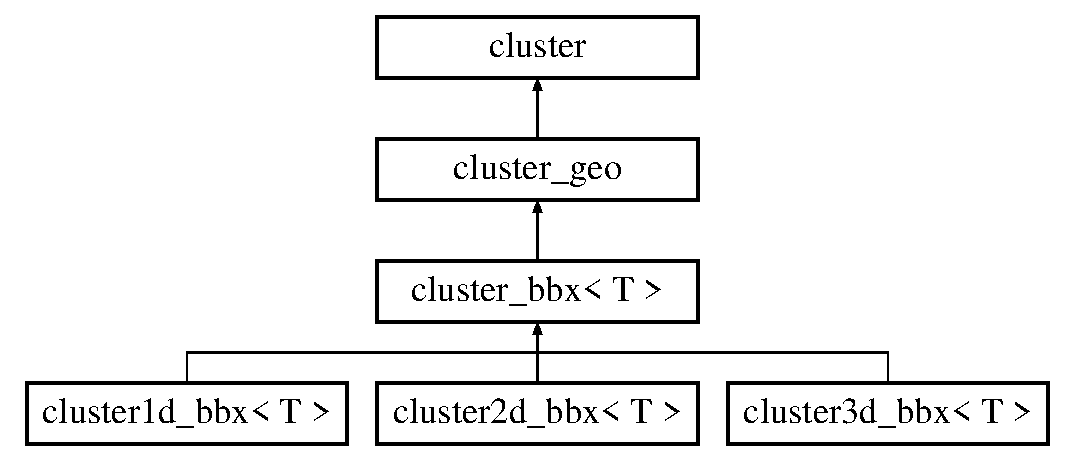
\includegraphics[height=4.000000cm]{classcluster__bbx}
\end{center}
\end{figure}
\subsection*{\-Public \-Member \-Functions}
\begin{DoxyCompactItemize}
\item 
virtual bool \hyperlink{classcluster__bbx_ab5852c7c8fb33c1b3a681c8f4b0eec10}{isadm} (double eta, \hyperlink{classcluster}{cluster} $\ast$cl, bl\-\_\-info \&info)=0
\item 
virtual void \hyperlink{classcluster__bbx_afa9ff45f3792189e25a46b8764f2da0c}{create\-Cluster\-Tree} (unsigned bmin, unsigned $\ast$op\-\_\-perm, unsigned $\ast$po\-\_\-perm)
\end{DoxyCompactItemize}


\subsection{\-Detailed \-Description}
\subsubsection*{template$<$class \-T$>$class cluster\-\_\-bbx$<$ T $>$}

\-A class for storing clusters of degrees of freedom. \-Subdivision is based on bounding boxes (bbx) 

\subsection{\-Member \-Function \-Documentation}
\hypertarget{classcluster__bbx_afa9ff45f3792189e25a46b8764f2da0c}{
\index{cluster\-\_\-bbx@{cluster\-\_\-bbx}!create\-Cluster\-Tree@{create\-Cluster\-Tree}}
\index{create\-Cluster\-Tree@{create\-Cluster\-Tree}!cluster_bbx@{cluster\-\_\-bbx}}
\subsubsection[{create\-Cluster\-Tree}]{\setlength{\rightskip}{0pt plus 5cm}template$<$class \-T$>$ virtual void {\bf cluster\-\_\-bbx}$<$ \-T $>$\-::create\-Cluster\-Tree (
\begin{DoxyParamCaption}
\item[{unsigned}]{bmin, }
\item[{unsigned $\ast$}]{op\-\_\-perm, }
\item[{unsigned $\ast$}]{po\-\_\-perm}
\end{DoxyParamCaption}
)\hspace{0.3cm}{\ttfamily  \mbox{[}inline, virtual\mbox{]}}}}
\label{classcluster__bbx_afa9ff45f3792189e25a46b8764f2da0c}
creates recursively the cluster tree, i.\-e. changes the permutation op\-\_\-perm and po\-\_\-perm and create child cluster trees 
\begin{DoxyParams}{\-Parameters}
{\em op\-\_\-perm} & permutation\-: permutated\-\_\-row = op\-\_\-perm\mbox{[}original\-\_\-row\mbox{]} \\
\hline
{\em po\-\_\-perm} & reverse permutation\-: original\-\_\-row = po\-\_\-perm\mbox{[}permutated\-\_\-idx\mbox{]} \\
\hline
{\em bmin} & threshold value for stopping further refinement \\
\hline
\end{DoxyParams}


\-Implements \hyperlink{classcluster_a7eb7a1209c0030e5cf344252f704fd57}{cluster}.



\-References cluster\-::create\-Cluster\-Tree(), and cluster\-::nbeg.

\hypertarget{classcluster__bbx_ab5852c7c8fb33c1b3a681c8f4b0eec10}{
\index{cluster\-\_\-bbx@{cluster\-\_\-bbx}!isadm@{isadm}}
\index{isadm@{isadm}!cluster_bbx@{cluster\-\_\-bbx}}
\subsubsection[{isadm}]{\setlength{\rightskip}{0pt plus 5cm}template$<$class \-T$>$ virtual bool {\bf cluster\-\_\-bbx}$<$ \-T $>$\-::isadm (
\begin{DoxyParamCaption}
\item[{double}]{eta2, }
\item[{{\bf cluster} $\ast$}]{cl, }
\item[{bl\-\_\-info \&}]{info}
\end{DoxyParamCaption}
)\hspace{0.3cm}{\ttfamily  \mbox{[}pure virtual\mbox{]}}}}
\label{classcluster__bbx_ab5852c7c8fb33c1b3a681c8f4b0eec10}
is this cluster admissible with the cluster cl ? bool\& only valid for cluster\-Sp\-N\-D 

\-Implements \hyperlink{classcluster_aa48a0f4aada61485263d76b82e819b4b}{cluster}.



\-Implemented in \hyperlink{classcluster3d__bbx_a435d59e2b633d01a2748b7353168796e}{cluster3d\-\_\-bbx$<$ T $>$}, \hyperlink{classcluster2d__bbx_a0c0e1d9841ed93b2a59b241fc68135e6}{cluster2d\-\_\-bbx$<$ T $>$}, and \hyperlink{classcluster1d__bbx_afbdd020333c05115e04969bef28db2cf}{cluster1d\-\_\-bbx$<$ T $>$}.



\-The documentation for this class was generated from the following file\-:\begin{DoxyCompactItemize}
\item 
cluster\-\_\-bbx.\-h\end{DoxyCompactItemize}

\hypertarget{classcluster__geo}{
\section{cluster\-\_\-geo \-Class \-Reference}
\label{classcluster__geo}\index{cluster\-\_\-geo@{cluster\-\_\-geo}}
}


basis class of a geometric cluster  




{\ttfamily \#include $<$cluster.\-h$>$}

\-Inheritance diagram for cluster\-\_\-geo\-:\begin{figure}[H]
\begin{center}
\leavevmode
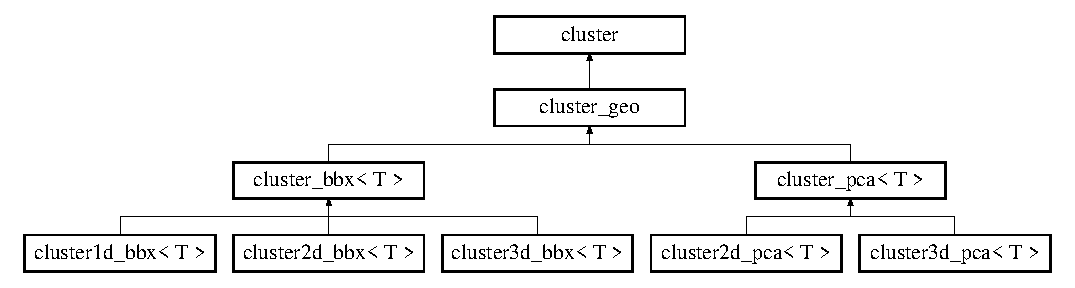
\includegraphics[height=3.419847cm]{classcluster__geo}
\end{center}
\end{figure}
\subsection*{\-Public \-Member \-Functions}
\begin{DoxyCompactItemize}
\item 
\hypertarget{classcluster__geo_a526263eed54fdc50ae80c8648a78e056}{
virtual unsigned \hyperlink{classcluster__geo_a526263eed54fdc50ae80c8648a78e056}{dim} () const =0}
\label{classcluster__geo_a526263eed54fdc50ae80c8648a78e056}

\begin{DoxyCompactList}\small\item\em returns the spatial dimension \end{DoxyCompactList}\end{DoxyCompactItemize}
\subsection*{\-Protected \-Attributes}
\begin{DoxyCompactItemize}
\item 
\hypertarget{classcluster__geo_a8e70ff925d9a1847985a2f63df8aa8ec}{
double \hyperlink{classcluster__geo_a8e70ff925d9a1847985a2f63df8aa8ec}{diam2}}
\label{classcluster__geo_a8e70ff925d9a1847985a2f63df8aa8ec}

\begin{DoxyCompactList}\small\item\em squared diameter \end{DoxyCompactList}\end{DoxyCompactItemize}


\subsection{\-Detailed \-Description}
basis class of a geometric cluster 

\-The documentation for this class was generated from the following file\-:\begin{DoxyCompactItemize}
\item 
\hyperlink{cluster_8h}{cluster.\-h}\end{DoxyCompactItemize}

\hypertarget{classcluster__pca}{
\section{cluster\-\_\-pca$<$ \-T $>$ \-Class \-Template \-Reference}
\label{classcluster__pca}\index{cluster\-\_\-pca$<$ T $>$@{cluster\-\_\-pca$<$ T $>$}}
}


\-A class for storing clusters of degrees of freedom. \-Subdivision is based on the principal component analysis (\-P\-C\-A)  




{\ttfamily \#include $<$cluster\-\_\-pca.\-h$>$}

\-Inheritance diagram for cluster\-\_\-pca$<$ \-T $>$\-:\begin{figure}[H]
\begin{center}
\leavevmode
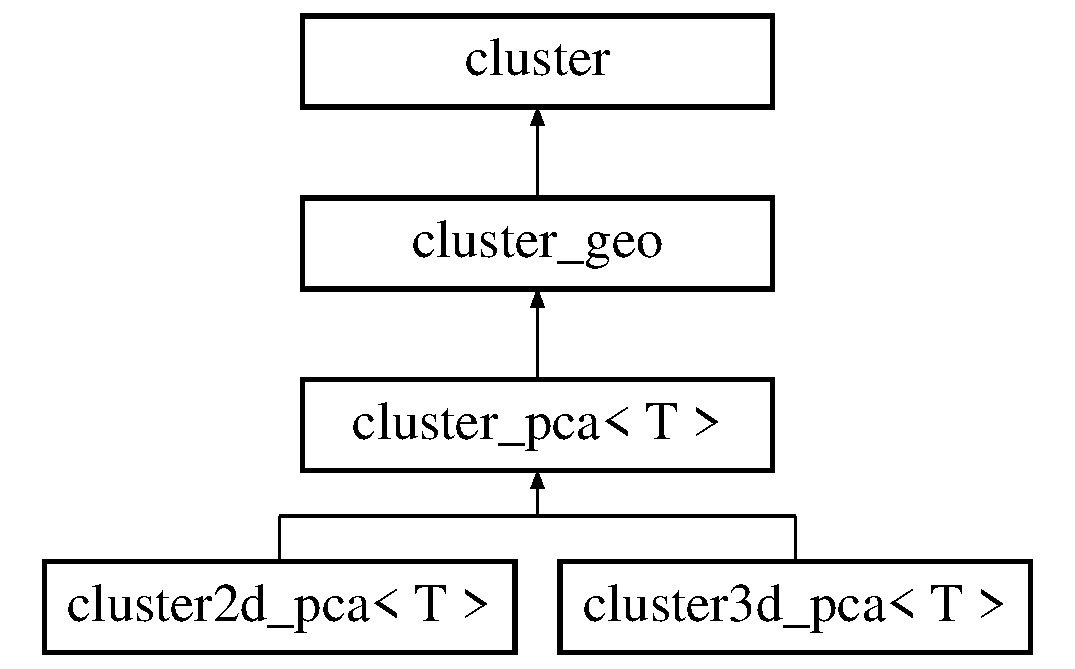
\includegraphics[height=4.000000cm]{classcluster__pca}
\end{center}
\end{figure}
\subsection*{\-Public \-Member \-Functions}
\begin{DoxyCompactItemize}
\item 
bool \hyperlink{classcluster__pca_a4546575a6d4e83e4d8ab6131019fae95}{isadm} (double eta2, \hyperlink{classcluster}{cluster} $\ast$cl, bl\-\_\-info \&info)
\item 
virtual void \hyperlink{classcluster__pca_a269105a7c9520bdcc566a858fbf6b763}{create\-Cluster\-Tree} (const unsigned bmin, unsigned $\ast$op\-\_\-perm, unsigned $\ast$po\-\_\-perm)
\end{DoxyCompactItemize}


\subsection{\-Detailed \-Description}
\subsubsection*{template$<$class \-T$>$class cluster\-\_\-pca$<$ T $>$}

\-A class for storing clusters of degrees of freedom. \-Subdivision is based on the principal component analysis (\-P\-C\-A) 

\subsection{\-Member \-Function \-Documentation}
\hypertarget{classcluster__pca_a269105a7c9520bdcc566a858fbf6b763}{
\index{cluster\-\_\-pca@{cluster\-\_\-pca}!create\-Cluster\-Tree@{create\-Cluster\-Tree}}
\index{create\-Cluster\-Tree@{create\-Cluster\-Tree}!cluster_pca@{cluster\-\_\-pca}}
\subsubsection[{create\-Cluster\-Tree}]{\setlength{\rightskip}{0pt plus 5cm}template$<$class \-T$>$ virtual void {\bf cluster\-\_\-pca}$<$ \-T $>$\-::create\-Cluster\-Tree (
\begin{DoxyParamCaption}
\item[{const unsigned}]{bmin, }
\item[{unsigned $\ast$}]{op\-\_\-perm, }
\item[{unsigned $\ast$}]{po\-\_\-perm}
\end{DoxyParamCaption}
)\hspace{0.3cm}{\ttfamily  \mbox{[}inline, virtual\mbox{]}}}}
\label{classcluster__pca_a269105a7c9520bdcc566a858fbf6b763}
creates recursively the cluster tree, i.\-e. changes the permutation op\-\_\-perm and po\-\_\-perm and create child cluster trees 
\begin{DoxyParams}{\-Parameters}
{\em op\-\_\-perm} & permutation\-: permutated\-\_\-row = op\-\_\-perm\mbox{[}original\-\_\-row\mbox{]} \\
\hline
{\em po\-\_\-perm} & reverse permutation\-: original\-\_\-row = po\-\_\-perm\mbox{[}permutated\-\_\-idx\mbox{]} \\
\hline
{\em bmin} & threshold value for stopping further refinement \\
\hline
\end{DoxyParams}


\-Implements \hyperlink{classcluster_a7eb7a1209c0030e5cf344252f704fd57}{cluster}.

\hypertarget{classcluster__pca_a4546575a6d4e83e4d8ab6131019fae95}{
\index{cluster\-\_\-pca@{cluster\-\_\-pca}!isadm@{isadm}}
\index{isadm@{isadm}!cluster_pca@{cluster\-\_\-pca}}
\subsubsection[{isadm}]{\setlength{\rightskip}{0pt plus 5cm}template$<$class \-T$>$ bool {\bf cluster\-\_\-pca}$<$ \-T $>$\-::isadm (
\begin{DoxyParamCaption}
\item[{double}]{eta2, }
\item[{{\bf cluster} $\ast$}]{cl, }
\item[{bl\-\_\-info \&}]{info}
\end{DoxyParamCaption}
)\hspace{0.3cm}{\ttfamily  \mbox{[}inline, virtual\mbox{]}}}}
\label{classcluster__pca_a4546575a6d4e83e4d8ab6131019fae95}
is this cluster admissible with the cluster cl ? bool\& only valid for cluster\-Sp\-N\-D 

\-Implements \hyperlink{classcluster_aa48a0f4aada61485263d76b82e819b4b}{cluster}.



\-The documentation for this class was generated from the following file\-:\begin{DoxyCompactItemize}
\item 
\hyperlink{cluster__pca_8h}{cluster\-\_\-pca.\-h}\end{DoxyCompactItemize}

\hypertarget{classcluster__ref}{
\section{cluster\-\_\-ref \-Class \-Reference}
\label{classcluster__ref}\index{cluster\-\_\-ref@{cluster\-\_\-ref}}
}


basis class for storing clusters with a reference to diagonal blocks  




{\ttfamily \#include $<$cluster.\-h$>$}

\-Inheritance diagram for cluster\-\_\-ref\-:\begin{figure}[H]
\begin{center}
\leavevmode
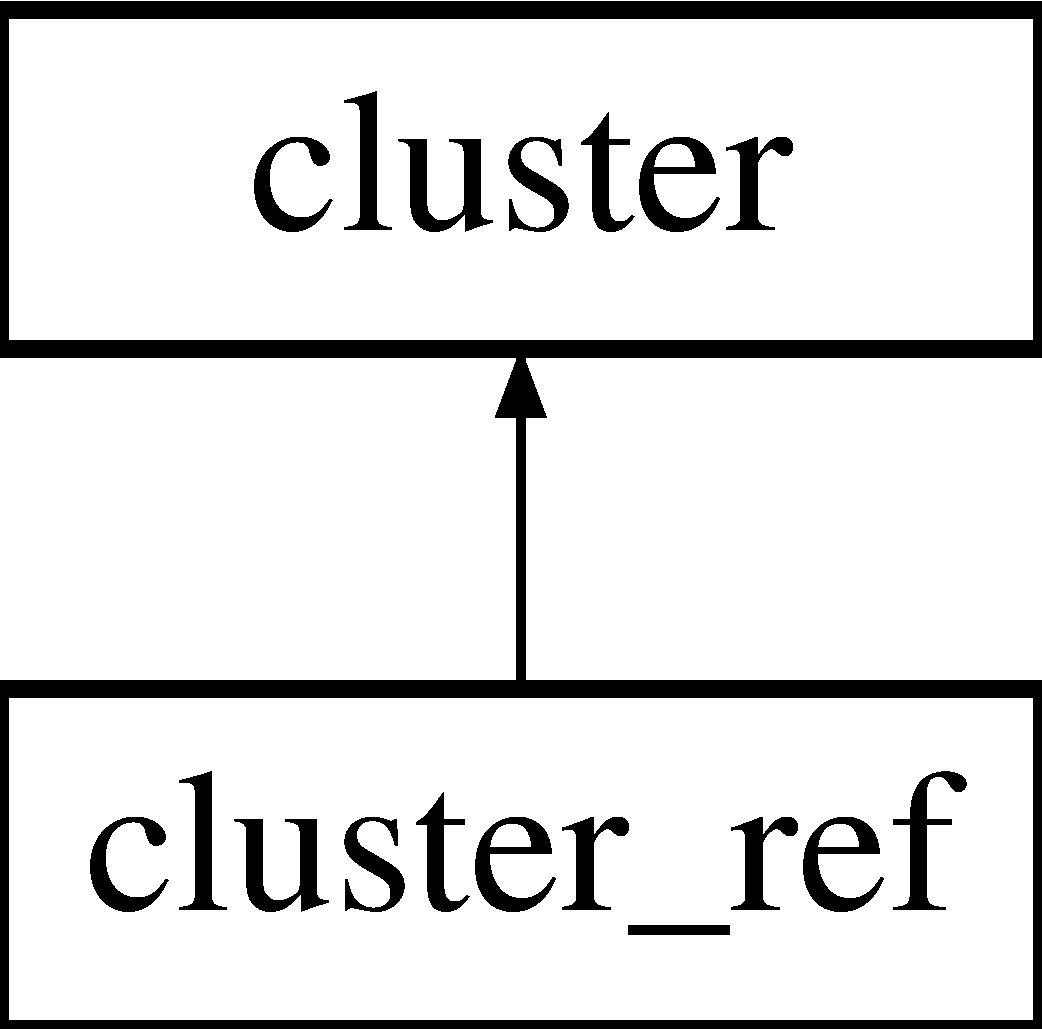
\includegraphics[height=2.000000cm]{classcluster__ref}
\end{center}
\end{figure}


\subsection{\-Detailed \-Description}
basis class for storing clusters with a reference to diagonal blocks 

\-The documentation for this class was generated from the following file\-:\begin{DoxyCompactItemize}
\item 
\hyperlink{cluster_8h}{cluster.\-h}\end{DoxyCompactItemize}

\hypertarget{classClusterAlg}{
\section{\-Cluster\-Alg \-Class \-Reference}
\label{classClusterAlg}\index{\-Cluster\-Alg@{\-Cluster\-Alg}}
}


\-Base class for storing clusters of degrees of freedom without geometric information.  




{\ttfamily \#include $<$\-Cluster\-Alg.\-h$>$}

\-Inheritance diagram for \-Cluster\-Alg\-:\begin{figure}[H]
\begin{center}
\leavevmode
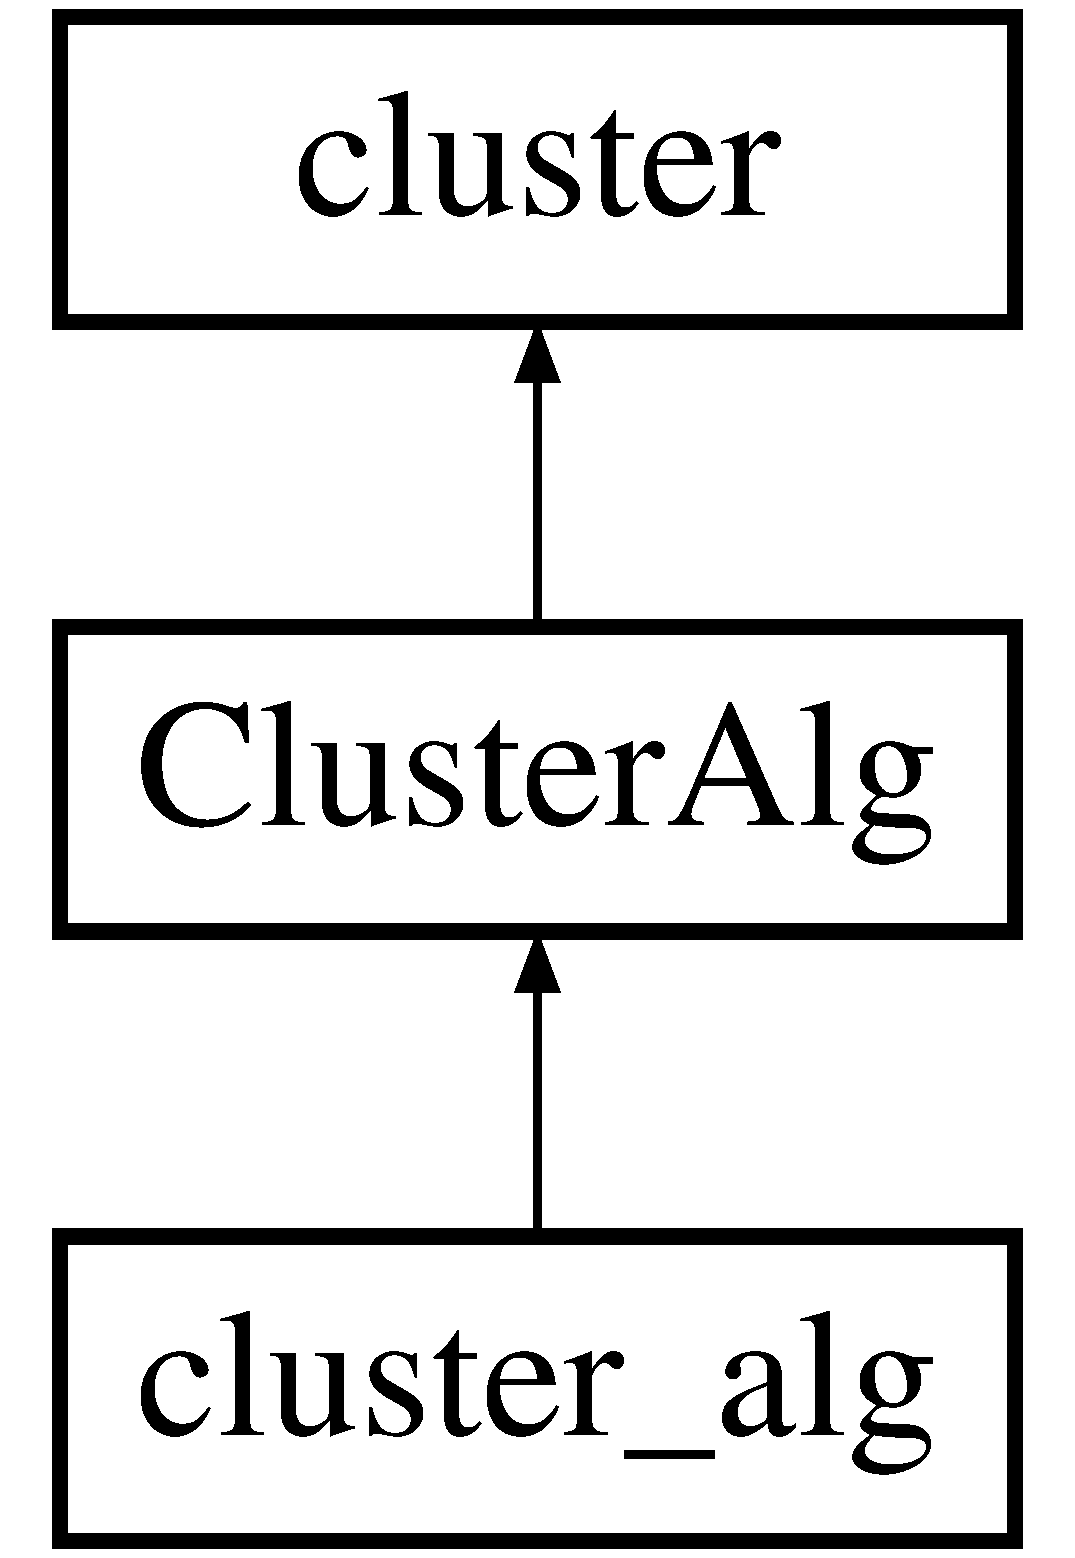
\includegraphics[height=3.000000cm]{classClusterAlg}
\end{center}
\end{figure}
\subsection*{\-Public \-Member \-Functions}
\begin{DoxyCompactItemize}
\item 
\hyperlink{classClusterAlg_a5637ecc2686cb0d43965470218e84863}{\-Cluster\-Alg} (unsigned n, unsigned $\ast$i\-A, unsigned $\ast$j\-A)
\item 
\hyperlink{classClusterAlg_a7cf98bcd418f6afdc30b7c7457722851}{\-Cluster\-Alg} (\hyperlink{classClusterAlg}{\-Cluster\-Alg} $\ast$father, unsigned beg, unsigned end, unsigned $\ast$\hyperlink{classClusterAlg_a4f06e1465978072d8c6bd098e062b701}{op\-\_\-perm}, unsigned $\ast$\hyperlink{classClusterAlg_af3d1d7c4ae0516ff9de725d3ff760b07}{po\-\_\-perm}, unsigned \hyperlink{classClusterAlg_ac06ccb0ba85be10e97392bd063fa78c8}{depth}, \-Adj\-Mat $\ast$global\-\_\-mat, \-Adj\-Mat $\ast$local\-\_\-mat)
\begin{DoxyCompactList}\small\item\em \-Constructor. \end{DoxyCompactList}\item 
\hypertarget{classClusterAlg_aa6496a6fbd35f3f230b9550778cb49c1}{
virtual \hyperlink{classClusterAlg_aa6496a6fbd35f3f230b9550778cb49c1}{$\sim$\-Cluster\-Alg} ()}
\label{classClusterAlg_aa6496a6fbd35f3f230b9550778cb49c1}

\begin{DoxyCompactList}\small\item\em \-Destructor. \-Destructor frees all form the objects allocated memory. \end{DoxyCompactList}\item 
virtual void \hyperlink{classClusterAlg_ab2615e5ba68257b11d477274737a9c52}{subdivide} (unsigned bmin)=0
\begin{DoxyCompactList}\small\item\em subdivide this cluster recursively, needed to generate the cluster tree \end{DoxyCompactList}\item 
virtual void \hyperlink{classClusterAlg_acbbefef10e2d91713a567af5bb5c08f7}{create\-Cluster\-Tree} (unsigned bmin, unsigned $\ast$\hyperlink{classClusterAlg_a4f06e1465978072d8c6bd098e062b701}{op\-\_\-perm}, unsigned $\ast$\hyperlink{classClusterAlg_af3d1d7c4ae0516ff9de725d3ff760b07}{po\-\_\-perm})
\item 
virtual void \hyperlink{classClusterAlg_a3da066d722da219e5f64f624a6121b05}{compute\-Neighbor} ()=0
\item 
unsigned \hyperlink{classClusterAlg_adce4fbafed2d9226336d3b57fae89692}{is\-Neighbour} (\hyperlink{classClusterAlg}{\-Cluster\-Alg} $\ast$const other, unsigned \&nnodes0, unsigned \&nnodes1) const 
\begin{DoxyCompactList}\small\item\em method checks if there exists edges in $(i, j) \in E(G(A))$ with $i$ in this cluster and $j$ in cluster other. \end{DoxyCompactList}\item 
void \hyperlink{classClusterAlg_ac7175d7df8045c8ad4363f709b5cc6cd}{neighbors\-To\-Array} ()
\item 
const std\-::list$<$ \-Neighbor $>$ \& \hyperlink{classClusterAlg_a468cf8819a9bae6a6b65db3ad6fb2d2d}{get\-Neighbor} () const 
\begin{DoxyCompactList}\small\item\em \-Method returns the list of \-Cluster\-Alg$\ast$ that are in the neighborhood of the actual \hyperlink{classClusterAlg}{\-Cluster\-Alg}. \end{DoxyCompactList}\item 
void \hyperlink{classClusterAlg_a3ce04d40392ab7e8143de5ffcaea6dda}{add\-Neighbor\-Element} (\-Neighbor b)
\item 
\hypertarget{classClusterAlg_a3daa14e294fe03b1405d057de3a640be}{
virtual bool \hyperlink{classClusterAlg_a3daa14e294fe03b1405d057de3a640be}{isadm} (double eta2, \hyperlink{classcluster}{cluster} $\ast$cl, bl\-\_\-info \&info)=0}
\label{classClusterAlg_a3daa14e294fe03b1405d057de3a640be}

\begin{DoxyCompactList}\small\item\em \-This method checks the admissibility of cluster this with the cluster cl. \end{DoxyCompactList}\item 
virtual bool \hyperlink{classClusterAlg_abe3332e66bad89111412fb0fa7928c66}{is\-Separator} () const =0
\item 
unsigned \hyperlink{classClusterAlg_ac21ad0586cca3b05c1df94fa66f224e4}{get\-Depth} () const 
\end{DoxyCompactItemize}
\subsection*{\-Protected \-Member \-Functions}
\begin{DoxyCompactItemize}
\item 
\hyperlink{classClusterAlg}{\-Cluster\-Alg} $\ast$ \hyperlink{classClusterAlg_a7b3c0f12a96e20016135ae5b98c100db}{get\-Parent} () const 
\begin{DoxyCompactList}\small\item\em \-Method returns the pointer to the parent cluster. \end{DoxyCompactList}\item 
unsigned \hyperlink{classClusterAlg_a1010355ccb56db6bc68b258e94c4a765}{has\-Neighbour} (\hyperlink{classClusterAlg}{\-Cluster\-Alg} $\ast$const other) const 
\end{DoxyCompactItemize}
\subsection*{\-Public \-Member \-Functions -\/ \-Graph related methods for}
\label{_amgrpd43883f7a3f1c1aa575f47a69a7c8e7b}%
 admissibility checking

\-The following methods base on graph-\/methods. \-The graph is generated with construct\-Graph from nodes consisting of cluster-\/tree-\/entities and edges between clusters if they are neighbored. \begin{DoxyCompactItemize}
\item 
\hyperlink{classClusterAlg}{\-Cluster\-Alg} $\ast$ \hyperlink{classClusterAlg_a1b63bc64e4622216b0539c4a5b76d3c2}{parent}
\item 
unsigned $\ast$ \hyperlink{classClusterAlg_a4f06e1465978072d8c6bd098e062b701}{op\-\_\-perm}
\item 
unsigned $\ast$ \hyperlink{classClusterAlg_af3d1d7c4ae0516ff9de725d3ff760b07}{po\-\_\-perm}
\item 
unsigned $\ast$ \hyperlink{classClusterAlg_a25fe84e1434812f52a484e14dc191a01}{\-\_\-l\-\_\-op\-\_\-perm}
\item 
unsigned $\ast$ \hyperlink{classClusterAlg_ae5aac25ca0791e244b25574814b18825}{\-\_\-l\-\_\-po\-\_\-perm}
\item 
unsigned \hyperlink{classClusterAlg_a38f91e914760de5e80a8023e5bb644bf}{diam}
\item 
unsigned \hyperlink{classClusterAlg_ac06ccb0ba85be10e97392bd063fa78c8}{depth}
\item 
\-Adj\-Mat $\ast$ \hyperlink{classClusterAlg_a29eb1ed447fe956fbece857e0ab898bc}{adj\-\_\-mat}
\item 
\-Adj\-Mat $\ast$ \hyperlink{classClusterAlg_aa7d43b82eac4084710cabafe6c9d8fee}{\-\_\-local\-\_\-adj\-\_\-mat}
\item 
std\-::list$<$ \-Neighbor $>$ \hyperlink{classClusterAlg_ace012e3a54a91c88fb486b7e02394d39}{list\-\_\-boundary}
\item 
\-Neighbor $\ast$ \hyperlink{classClusterAlg_a09156a9cf7570cde252131f25e599fbb}{neighbors}
\item 
unsigned \hyperlink{classClusterAlg_af1b22f77639a805d28569806d561600e}{nneighbors}
\item 
unsigned \hyperlink{classClusterAlg_ac1034ff983ce968e11edaf18c2b15cb2}{vdepth}
\item 
\-M\-Graph$<$ \hyperlink{classClusterAlg}{\-Cluster\-Alg} $\ast$, unsigned $>$ $\ast$ \hyperlink{classClusterAlg_ad3a53cf9fb7af4e2a45e7d859bc87c7b}{construct\-Graph} (\hyperlink{classClusterAlg}{\-Cluster\-Alg} $\ast$t\-\_\-2, unsigned up=0)
\begin{DoxyCompactList}\small\item\em \-Method computes an estimation of the distance between the cluster represented by this object and the cluster other based on graphs for the admissibility check. \end{DoxyCompactList}\item 
void \hyperlink{classClusterAlg_a108b12bb473f429c897e7ba004dd8b62}{find\-Roots} (\hyperlink{classClusterAlg}{\-Cluster\-Alg} $\ast$\&p\-\_\-0, \hyperlink{classClusterAlg}{\-Cluster\-Alg} $\ast$\&p\-\_\-1) const 
\begin{DoxyCompactList}\small\item\em \-Method find\-Roots returns first neighbored pair of predecessors in the cluster tree. \end{DoxyCompactList}\item 
void \hyperlink{classClusterAlg_ab4050fdfb42dc0ebec40c7464bbaf4ab}{get\-Nodes} (unsigned level, std\-::list$<$ \hyperlink{classClusterAlg}{\-Cluster\-Alg} $\ast$ $>$ \&nodes)
\begin{DoxyCompactList}\small\item\em \-Method traverses recursively the cluster-\/tree until a given level. \-If this level is achieved the pointer to this cluster is inserted into the list. \end{DoxyCompactList}\item 
\hypertarget{classClusterAlg_aa2c3643c9a48e40c8adb7acbd3011ec5}{
unsigned \hyperlink{classClusterAlg_aa2c3643c9a48e40c8adb7acbd3011ec5}{get\-Diam} () const }
\label{classClusterAlg_aa2c3643c9a48e40c8adb7acbd3011ec5}

\begin{DoxyCompactList}\small\item\em method returns an estimation of the diameter of the cluster. for the estimation holds\-: radius of graph $<$= estimated diam $<$= diameter of graph the value is computed in the constructor \end{DoxyCompactList}\item 
\hypertarget{classClusterAlg_abef00c7a121ff7af20898688e2a2d3db}{
void {\bfseries set\-Diam} (unsigned d)}
\label{classClusterAlg_abef00c7a121ff7af20898688e2a2d3db}

\item 
\hypertarget{classClusterAlg_ac25fcff58a42fd7703320154a7fa237b}{
unsigned {\bfseries get\-Virtual\-Depth} () const }
\label{classClusterAlg_ac25fcff58a42fd7703320154a7fa237b}

\item 
\hypertarget{classClusterAlg_ad04c66e0c57ef73831a87ce6b5e98d96}{
void {\bfseries set\-Virtual\-Depth} (unsigned vd)}
\label{classClusterAlg_ad04c66e0c57ef73831a87ce6b5e98d96}

\item 
\hypertarget{classClusterAlg_ad1b8fae8a667f970373e9d20b99e335e}{
virtual void {\bfseries refine} (unsigned max\-\_\-level)=0}
\label{classClusterAlg_ad1b8fae8a667f970373e9d20b99e335e}

\end{DoxyCompactItemize}


\subsection{\-Detailed \-Description}
\-Base class for storing clusters of degrees of freedom without geometric information. 

\subsection{\-Constructor \& \-Destructor \-Documentation}
\hypertarget{classClusterAlg_a5637ecc2686cb0d43965470218e84863}{
\index{\-Cluster\-Alg@{\-Cluster\-Alg}!\-Cluster\-Alg@{\-Cluster\-Alg}}
\index{\-Cluster\-Alg@{\-Cluster\-Alg}!ClusterAlg@{\-Cluster\-Alg}}
\subsubsection[{\-Cluster\-Alg}]{\setlength{\rightskip}{0pt plus 5cm}\-Cluster\-Alg\-::\-Cluster\-Alg (
\begin{DoxyParamCaption}
\item[{unsigned}]{n, }
\item[{unsigned $\ast$}]{i\-A, }
\item[{unsigned $\ast$}]{j\-A}
\end{DoxyParamCaption}
)}}
\label{classClusterAlg_a5637ecc2686cb0d43965470218e84863}
\-Constructor creates the root of the cluster tree 
\begin{DoxyParams}{\-Parameters}
{\em n} & \\
\hline
{\em i\-A} & \\
\hline
{\em j\-A} & \\
\hline
\end{DoxyParams}
\begin{DoxyReturn}{\-Returns}

\end{DoxyReturn}
\hypertarget{classClusterAlg_a7cf98bcd418f6afdc30b7c7457722851}{
\index{\-Cluster\-Alg@{\-Cluster\-Alg}!\-Cluster\-Alg@{\-Cluster\-Alg}}
\index{\-Cluster\-Alg@{\-Cluster\-Alg}!ClusterAlg@{\-Cluster\-Alg}}
\subsubsection[{\-Cluster\-Alg}]{\setlength{\rightskip}{0pt plus 5cm}\-Cluster\-Alg\-::\-Cluster\-Alg (
\begin{DoxyParamCaption}
\item[{{\bf \-Cluster\-Alg} $\ast$}]{father, }
\item[{unsigned}]{beg, }
\item[{unsigned}]{end, }
\item[{unsigned $\ast$}]{op\-\_\-perm, }
\item[{unsigned $\ast$}]{po\-\_\-perm, }
\item[{unsigned}]{depth, }
\item[{\-Adj\-Mat $\ast$}]{global\-\_\-mat, }
\item[{\-Adj\-Mat $\ast$}]{local\-\_\-mat}
\end{DoxyParamCaption}
)}}
\label{classClusterAlg_a7cf98bcd418f6afdc30b7c7457722851}


\-Constructor. 


\begin{DoxyParams}{\-Parameters}
{\em father} & parent node in cluster tree \\
\hline
{\em beg} & beginning index of the cluster (see class \-D\-O\-F\-Point) \\
\hline
{\em end} & beginning index of the next cluster (see class \-D\-O\-F\-Point) \\
\hline
{\em op\-\_\-perm} & \\
\hline
{\em po\-\_\-perm} & \\
\hline
{\em depth} & distance between this node and the root \\
\hline
{\em global\-\_\-mat} & reference to the global adjacency matrix of the matrix graph in crs format \\
\hline
{\em local\-\_\-mat} & pointer to the local adjacency matrix of the matrix graph in crs format format \\
\hline
\end{DoxyParams}


\subsection{\-Member \-Function \-Documentation}
\hypertarget{classClusterAlg_a3ce04d40392ab7e8143de5ffcaea6dda}{
\index{\-Cluster\-Alg@{\-Cluster\-Alg}!add\-Neighbor\-Element@{add\-Neighbor\-Element}}
\index{add\-Neighbor\-Element@{add\-Neighbor\-Element}!ClusterAlg@{\-Cluster\-Alg}}
\subsubsection[{add\-Neighbor\-Element}]{\setlength{\rightskip}{0pt plus 5cm}void \-Cluster\-Alg\-::add\-Neighbor\-Element (
\begin{DoxyParamCaption}
\item[{\-Neighbor}]{b}
\end{DoxyParamCaption}
)\hspace{0.3cm}{\ttfamily  \mbox{[}inline\mbox{]}}}}
\label{classClusterAlg_a3ce04d40392ab7e8143de5ffcaea6dda}
\-Method adds \-Cluster or \-Separator to the boundary of the actual cluster. 

\-References list\-\_\-boundary.

\hypertarget{classClusterAlg_a3da066d722da219e5f64f624a6121b05}{
\index{\-Cluster\-Alg@{\-Cluster\-Alg}!compute\-Neighbor@{compute\-Neighbor}}
\index{compute\-Neighbor@{compute\-Neighbor}!ClusterAlg@{\-Cluster\-Alg}}
\subsubsection[{compute\-Neighbor}]{\setlength{\rightskip}{0pt plus 5cm}virtual void \-Cluster\-Alg\-::compute\-Neighbor (
\begin{DoxyParamCaption}
{}
\end{DoxyParamCaption}
)\hspace{0.3cm}{\ttfamily  \mbox{[}pure virtual\mbox{]}}}}
\label{classClusterAlg_a3da066d722da219e5f64f624a6121b05}
\-Method traverses the \-Cluster\-Alg-\/tree and computes the boundary clusters of the actual cluster. 

\-Implemented in \hyperlink{classcluster__alg_a78292c11a717fb5b83762fc4c070797f}{cluster\-\_\-alg}.

\hypertarget{classClusterAlg_ad3a53cf9fb7af4e2a45e7d859bc87c7b}{
\index{\-Cluster\-Alg@{\-Cluster\-Alg}!construct\-Graph@{construct\-Graph}}
\index{construct\-Graph@{construct\-Graph}!ClusterAlg@{\-Cluster\-Alg}}
\subsubsection[{construct\-Graph}]{\setlength{\rightskip}{0pt plus 5cm}\-M\-Graph$<${\bf \-Cluster\-Alg}$\ast$, unsigned$>$$\ast$ \-Cluster\-Alg\-::construct\-Graph (
\begin{DoxyParamCaption}
\item[{{\bf \-Cluster\-Alg} $\ast$}]{t\-\_\-2, }
\item[{unsigned}]{up = {\ttfamily 0}}
\end{DoxyParamCaption}
)}}
\label{classClusterAlg_ad3a53cf9fb7af4e2a45e7d859bc87c7b}


\-Method computes an estimation of the distance between the cluster represented by this object and the cluster other based on graphs for the admissibility check. 

\-In order to compute the estimation get\-Dist() sets up a graph and uses the algorithm of \-Dijkstra to compute the distance, whereas the graph is build by method \hyperlink{classClusterAlg_ad3a53cf9fb7af4e2a45e7d859bc87c7b}{construct\-Graph()}. 
\begin{DoxyParams}{\-Parameters}
{\em other} & cluster object to whom distance should be computed \\
\hline
\end{DoxyParams}
\begin{DoxyReturn}{\-Returns}
distance in the graph\-Method construct\-Graph constructs the graph \$\-G\-\_\-\-D\$. \-For this purpose two neighbored predecessors \$p\-\_\-0, p\-\_\-1  \-T\-\_\-\-I\$ are searched using \hyperlink{classClusterAlg_a108b12bb473f429c897e7ba004dd8b62}{find\-Roots()}. \-All clusters rooted at \$p\-\_\-0, p\-\_\-1\$ in the actual level are collected in a list by \hyperlink{classClusterAlg_ab4050fdfb42dc0ebec40c7464bbaf4ab}{get\-Nodes()}. \-These are the vertices of \$\-G\-\_\-\-D\$. \-Two vertices are neighbored iff the clusters are neighbored. \-The weight of an edge is difference between the actual level and the virtual level. 
\end{DoxyReturn}

\begin{DoxyParams}{\-Parameters}
{\em other} & an other cluster for the block \$b = this  t\-\_\-2\$ \\
\hline
\end{DoxyParams}
\begin{DoxyReturn}{\-Returns}
a simple weighted graph 
\end{DoxyReturn}
\hypertarget{classClusterAlg_acbbefef10e2d91713a567af5bb5c08f7}{
\index{\-Cluster\-Alg@{\-Cluster\-Alg}!create\-Cluster\-Tree@{create\-Cluster\-Tree}}
\index{create\-Cluster\-Tree@{create\-Cluster\-Tree}!ClusterAlg@{\-Cluster\-Alg}}
\subsubsection[{create\-Cluster\-Tree}]{\setlength{\rightskip}{0pt plus 5cm}virtual void \-Cluster\-Alg\-::create\-Cluster\-Tree (
\begin{DoxyParamCaption}
\item[{unsigned}]{bmin, }
\item[{unsigned $\ast$}]{op\-\_\-perm, }
\item[{unsigned $\ast$}]{po\-\_\-perm}
\end{DoxyParamCaption}
)\hspace{0.3cm}{\ttfamily  \mbox{[}inline, virtual\mbox{]}}}}
\label{classClusterAlg_acbbefef10e2d91713a567af5bb5c08f7}
\-Method creates recursively the cluster tree, i.\-e. changes the permutation op\-\_\-perm and po\-\_\-perm and create child cluster trees. \-For this task only the adjacency matrix is used. 
\begin{DoxyParams}{\-Parameters}
{\em op\-\_\-perm} & permutation\-: permutated\-\_\-row = op\-\_\-perm\mbox{[}original\-\_\-row\mbox{]} \\
\hline
{\em po\-\_\-perm} & reverse permutation\-: original\-\_\-row = po\-\_\-perm\mbox{[}permutated\-\_\-idx\mbox{]} \\
\hline
{\em bmin} & threshold value for stopping further refinement \\
\hline
\end{DoxyParams}
\begin{DoxyReturn}{\-Returns}
a cluster tree 
\end{DoxyReturn}


\-Implements \hyperlink{classcluster_a7eb7a1209c0030e5cf344252f704fd57}{cluster}.



\-Reimplemented in \hyperlink{classcluster__alg_a2464aa83e8604d2098870c461f93b013}{cluster\-\_\-alg}.

\hypertarget{classClusterAlg_a108b12bb473f429c897e7ba004dd8b62}{
\index{\-Cluster\-Alg@{\-Cluster\-Alg}!find\-Roots@{find\-Roots}}
\index{find\-Roots@{find\-Roots}!ClusterAlg@{\-Cluster\-Alg}}
\subsubsection[{find\-Roots}]{\setlength{\rightskip}{0pt plus 5cm}void \-Cluster\-Alg\-::find\-Roots (
\begin{DoxyParamCaption}
\item[{{\bf \-Cluster\-Alg} $\ast$\&}]{p\-\_\-0, }
\item[{{\bf \-Cluster\-Alg} $\ast$\&}]{p\-\_\-1}
\end{DoxyParamCaption}
) const}}
\label{classClusterAlg_a108b12bb473f429c897e7ba004dd8b62}


\-Method find\-Roots returns first neighbored pair of predecessors in the cluster tree. 


\begin{DoxyParams}{\-Parameters}
{\em \$p\-\_\-0\$} & input\-: the starting cluster, output\-: the predecessor neighbored with a predecessor of \$p\-\_\-1\$ \\
\hline
{\em \$p\-\_\-1\$} & input\-: the starting cluster, output\-: the predecessor neighbored with a predecessor of \$p\-\_\-0\$ \\
\hline
\end{DoxyParams}
\hypertarget{classClusterAlg_ac21ad0586cca3b05c1df94fa66f224e4}{
\index{\-Cluster\-Alg@{\-Cluster\-Alg}!get\-Depth@{get\-Depth}}
\index{get\-Depth@{get\-Depth}!ClusterAlg@{\-Cluster\-Alg}}
\subsubsection[{get\-Depth}]{\setlength{\rightskip}{0pt plus 5cm}unsigned \-Cluster\-Alg\-::get\-Depth (
\begin{DoxyParamCaption}
{}
\end{DoxyParamCaption}
) const\hspace{0.3cm}{\ttfamily  \mbox{[}inline\mbox{]}}}}
\label{classClusterAlg_ac21ad0586cca3b05c1df94fa66f224e4}
\-The attribute depth takes the position of this cluster into the cluster-\/tree. \begin{DoxyReturn}{\-Returns}
the value of depth 
\end{DoxyReturn}


\-References depth.

\hypertarget{classClusterAlg_a468cf8819a9bae6a6b65db3ad6fb2d2d}{
\index{\-Cluster\-Alg@{\-Cluster\-Alg}!get\-Neighbor@{get\-Neighbor}}
\index{get\-Neighbor@{get\-Neighbor}!ClusterAlg@{\-Cluster\-Alg}}
\subsubsection[{get\-Neighbor}]{\setlength{\rightskip}{0pt plus 5cm}const std\-::list$<$\-Neighbor$>$\& \-Cluster\-Alg\-::get\-Neighbor (
\begin{DoxyParamCaption}
{}
\end{DoxyParamCaption}
) const\hspace{0.3cm}{\ttfamily  \mbox{[}inline\mbox{]}}}}
\label{classClusterAlg_a468cf8819a9bae6a6b65db3ad6fb2d2d}


\-Method returns the list of \-Cluster\-Alg$\ast$ that are in the neighborhood of the actual \hyperlink{classClusterAlg}{\-Cluster\-Alg}. 

\begin{DoxyReturn}{\-Returns}
the boundary of the actual cluster 
\end{DoxyReturn}


\-References list\-\_\-boundary.

\hypertarget{classClusterAlg_ab4050fdfb42dc0ebec40c7464bbaf4ab}{
\index{\-Cluster\-Alg@{\-Cluster\-Alg}!get\-Nodes@{get\-Nodes}}
\index{get\-Nodes@{get\-Nodes}!ClusterAlg@{\-Cluster\-Alg}}
\subsubsection[{get\-Nodes}]{\setlength{\rightskip}{0pt plus 5cm}void \-Cluster\-Alg\-::get\-Nodes (
\begin{DoxyParamCaption}
\item[{unsigned}]{level, }
\item[{std\-::list$<$ {\bf \-Cluster\-Alg} $\ast$ $>$ \&}]{nodes}
\end{DoxyParamCaption}
)}}
\label{classClusterAlg_ab4050fdfb42dc0ebec40c7464bbaf4ab}


\-Method traverses recursively the cluster-\/tree until a given level. \-If this level is achieved the pointer to this cluster is inserted into the list. 


\begin{DoxyParams}{\-Parameters}
{\em nodes} & the list of pointers to the appropriate clusters (output) \\
\hline
\end{DoxyParams}
\hypertarget{classClusterAlg_a7b3c0f12a96e20016135ae5b98c100db}{
\index{\-Cluster\-Alg@{\-Cluster\-Alg}!get\-Parent@{get\-Parent}}
\index{get\-Parent@{get\-Parent}!ClusterAlg@{\-Cluster\-Alg}}
\subsubsection[{get\-Parent}]{\setlength{\rightskip}{0pt plus 5cm}{\bf \-Cluster\-Alg}$\ast$ \-Cluster\-Alg\-::get\-Parent (
\begin{DoxyParamCaption}
{}
\end{DoxyParamCaption}
) const\hspace{0.3cm}{\ttfamily  \mbox{[}inline, protected\mbox{]}}}}
\label{classClusterAlg_a7b3c0f12a96e20016135ae5b98c100db}


\-Method returns the pointer to the parent cluster. 

\begin{DoxyReturn}{\-Returns}
parent cluster 
\end{DoxyReturn}


\-References parent.

\hypertarget{classClusterAlg_a1010355ccb56db6bc68b258e94c4a765}{
\index{\-Cluster\-Alg@{\-Cluster\-Alg}!has\-Neighbour@{has\-Neighbour}}
\index{has\-Neighbour@{has\-Neighbour}!ClusterAlg@{\-Cluster\-Alg}}
\subsubsection[{has\-Neighbour}]{\setlength{\rightskip}{0pt plus 5cm}unsigned \-Cluster\-Alg\-::has\-Neighbour (
\begin{DoxyParamCaption}
\item[{{\bf \-Cluster\-Alg} $\ast$const}]{other}
\end{DoxyParamCaption}
) const\hspace{0.3cm}{\ttfamily  \mbox{[}protected\mbox{]}}}}
\label{classClusterAlg_a1010355ccb56db6bc68b258e94c4a765}
has\-Neighbour iterates through the boundary list searching for pointer to other 
\begin{DoxyParams}{\-Parameters}
{\em other} & the \hyperlink{classClusterAlg}{\-Cluster\-Alg} to check with \\
\hline
\end{DoxyParams}
\begin{DoxyReturn}{\-Returns}
the size of neighbour 
\end{DoxyReturn}
\hypertarget{classClusterAlg_adce4fbafed2d9226336d3b57fae89692}{
\index{\-Cluster\-Alg@{\-Cluster\-Alg}!is\-Neighbour@{is\-Neighbour}}
\index{is\-Neighbour@{is\-Neighbour}!ClusterAlg@{\-Cluster\-Alg}}
\subsubsection[{is\-Neighbour}]{\setlength{\rightskip}{0pt plus 5cm}unsigned \-Cluster\-Alg\-::is\-Neighbour (
\begin{DoxyParamCaption}
\item[{{\bf \-Cluster\-Alg} $\ast$const}]{other, }
\item[{unsigned \&}]{nnodes0, }
\item[{unsigned \&}]{nnodes1}
\end{DoxyParamCaption}
) const}}
\label{classClusterAlg_adce4fbafed2d9226336d3b57fae89692}


method checks if there exists edges in $(i, j) \in E(G(A))$ with $i$ in this cluster and $j$ in cluster other. 


\begin{DoxyParams}{\-Parameters}
{\em input,\-:} & other \hyperlink{classClusterAlg}{\-Cluster\-Alg} object, in particular the represented index set \\
\hline
{\em nnodes0} & output\-: number of nodes in this cluster adjacent with any node into the other cluster \\
\hline
{\em nnodes1} & output\-: number of nodes in other cluster adjacent with any node into this cluster \\
\hline
\end{DoxyParams}
\begin{DoxyReturn}{\-Returns}
the number of edges between the clusters 
\end{DoxyReturn}
\hypertarget{classClusterAlg_abe3332e66bad89111412fb0fa7928c66}{
\index{\-Cluster\-Alg@{\-Cluster\-Alg}!is\-Separator@{is\-Separator}}
\index{is\-Separator@{is\-Separator}!ClusterAlg@{\-Cluster\-Alg}}
\subsubsection[{is\-Separator}]{\setlength{\rightskip}{0pt plus 5cm}virtual bool \-Cluster\-Alg\-::is\-Separator (
\begin{DoxyParamCaption}
{}
\end{DoxyParamCaption}
) const\hspace{0.3cm}{\ttfamily  \mbox{[}pure virtual\mbox{]}}}}
\label{classClusterAlg_abe3332e66bad89111412fb0fa7928c66}
\-Method returns the status of this \hyperlink{classClusterAlg}{\-Cluster\-Alg} object. 

\-Implemented in \hyperlink{classcluster__alg_a20b9fac849beaf8b760e3bb15fae66e0}{cluster\-\_\-alg}.

\hypertarget{classClusterAlg_ac7175d7df8045c8ad4363f709b5cc6cd}{
\index{\-Cluster\-Alg@{\-Cluster\-Alg}!neighbors\-To\-Array@{neighbors\-To\-Array}}
\index{neighbors\-To\-Array@{neighbors\-To\-Array}!ClusterAlg@{\-Cluster\-Alg}}
\subsubsection[{neighbors\-To\-Array}]{\setlength{\rightskip}{0pt plus 5cm}void \-Cluster\-Alg\-::neighbors\-To\-Array (
\begin{DoxyParamCaption}
{}
\end{DoxyParamCaption}
)}}
\label{classClusterAlg_ac7175d7df8045c8ad4363f709b5cc6cd}
transforms the list of neighbors into a sorted array of neighbors \hypertarget{classClusterAlg_ab2615e5ba68257b11d477274737a9c52}{
\index{\-Cluster\-Alg@{\-Cluster\-Alg}!subdivide@{subdivide}}
\index{subdivide@{subdivide}!ClusterAlg@{\-Cluster\-Alg}}
\subsubsection[{subdivide}]{\setlength{\rightskip}{0pt plus 5cm}virtual void \-Cluster\-Alg\-::subdivide (
\begin{DoxyParamCaption}
\item[{unsigned}]{bmin}
\end{DoxyParamCaption}
)\hspace{0.3cm}{\ttfamily  \mbox{[}pure virtual\mbox{]}}}}
\label{classClusterAlg_ab2615e5ba68257b11d477274737a9c52}


subdivide this cluster recursively, needed to generate the cluster tree 

only for compatibility. empty implementation. 
\begin{DoxyParams}{\-Parameters}
{\em @param} & \\
\hline
{\em $\backslash$param} & bmin the minimal size of clusters (input) \\
\hline
\end{DoxyParams}


\-Implemented in \hyperlink{classcluster__alg_a411de6be2059e0c2848c4b11f9a043cf}{cluster\-\_\-alg}.



\subsection{\-Member \-Data \-Documentation}
\hypertarget{classClusterAlg_a25fe84e1434812f52a484e14dc191a01}{
\index{\-Cluster\-Alg@{\-Cluster\-Alg}!\-\_\-l\-\_\-op\-\_\-perm@{\-\_\-l\-\_\-op\-\_\-perm}}
\index{\-\_\-l\-\_\-op\-\_\-perm@{\-\_\-l\-\_\-op\-\_\-perm}!ClusterAlg@{\-Cluster\-Alg}}
\subsubsection[{\-\_\-l\-\_\-op\-\_\-perm}]{\setlength{\rightskip}{0pt plus 5cm}unsigned$\ast$ {\bf \-Cluster\-Alg\-::\-\_\-l\-\_\-op\-\_\-perm}\hspace{0.3cm}{\ttfamily  \mbox{[}protected\mbox{]}}}}
\label{classClusterAlg_a25fe84e1434812f52a484e14dc191a01}
local permutation\-: original $<$-\/ l\-\_\-op\-\_\-perm $<$-\/ permutation \hypertarget{classClusterAlg_ae5aac25ca0791e244b25574814b18825}{
\index{\-Cluster\-Alg@{\-Cluster\-Alg}!\-\_\-l\-\_\-po\-\_\-perm@{\-\_\-l\-\_\-po\-\_\-perm}}
\index{\-\_\-l\-\_\-po\-\_\-perm@{\-\_\-l\-\_\-po\-\_\-perm}!ClusterAlg@{\-Cluster\-Alg}}
\subsubsection[{\-\_\-l\-\_\-po\-\_\-perm}]{\setlength{\rightskip}{0pt plus 5cm}unsigned$\ast$ {\bf \-Cluster\-Alg\-::\-\_\-l\-\_\-po\-\_\-perm}\hspace{0.3cm}{\ttfamily  \mbox{[}protected\mbox{]}}}}
\label{classClusterAlg_ae5aac25ca0791e244b25574814b18825}
local permutation\-: permutation $<$-\/ l\-\_\-po\-\_\-perm $<$-\/ original \hypertarget{classClusterAlg_aa7d43b82eac4084710cabafe6c9d8fee}{
\index{\-Cluster\-Alg@{\-Cluster\-Alg}!\-\_\-local\-\_\-adj\-\_\-mat@{\-\_\-local\-\_\-adj\-\_\-mat}}
\index{\-\_\-local\-\_\-adj\-\_\-mat@{\-\_\-local\-\_\-adj\-\_\-mat}!ClusterAlg@{\-Cluster\-Alg}}
\subsubsection[{\-\_\-local\-\_\-adj\-\_\-mat}]{\setlength{\rightskip}{0pt plus 5cm}\-Adj\-Mat$\ast$ {\bf \-Cluster\-Alg\-::\-\_\-local\-\_\-adj\-\_\-mat}\hspace{0.3cm}{\ttfamily  \mbox{[}protected\mbox{]}}}}
\label{classClusterAlg_aa7d43b82eac4084710cabafe6c9d8fee}
local adjacency matrix \hypertarget{classClusterAlg_a29eb1ed447fe956fbece857e0ab898bc}{
\index{\-Cluster\-Alg@{\-Cluster\-Alg}!adj\-\_\-mat@{adj\-\_\-mat}}
\index{adj\-\_\-mat@{adj\-\_\-mat}!ClusterAlg@{\-Cluster\-Alg}}
\subsubsection[{adj\-\_\-mat}]{\setlength{\rightskip}{0pt plus 5cm}\-Adj\-Mat$\ast$ {\bf \-Cluster\-Alg\-::adj\-\_\-mat}\hspace{0.3cm}{\ttfamily  \mbox{[}protected\mbox{]}}}}
\label{classClusterAlg_a29eb1ed447fe956fbece857e0ab898bc}
\-The \-Adj\-Mat stores the edge set of the matrix graph \$\-G = (\-V,\-E)\$. (see class \-Adj\-Mat) \hypertarget{classClusterAlg_ac06ccb0ba85be10e97392bd063fa78c8}{
\index{\-Cluster\-Alg@{\-Cluster\-Alg}!depth@{depth}}
\index{depth@{depth}!ClusterAlg@{\-Cluster\-Alg}}
\subsubsection[{depth}]{\setlength{\rightskip}{0pt plus 5cm}unsigned {\bf \-Cluster\-Alg\-::depth}\hspace{0.3cm}{\ttfamily  \mbox{[}protected\mbox{]}}}}
\label{classClusterAlg_ac06ccb0ba85be10e97392bd063fa78c8}
distance between the root node and this cluster 

\-Referenced by get\-Depth().

\hypertarget{classClusterAlg_a38f91e914760de5e80a8023e5bb644bf}{
\index{\-Cluster\-Alg@{\-Cluster\-Alg}!diam@{diam}}
\index{diam@{diam}!ClusterAlg@{\-Cluster\-Alg}}
\subsubsection[{diam}]{\setlength{\rightskip}{0pt plus 5cm}unsigned {\bf \-Cluster\-Alg\-::diam}\hspace{0.3cm}{\ttfamily  \mbox{[}protected\mbox{]}}}}
\label{classClusterAlg_a38f91e914760de5e80a8023e5bb644bf}
approximation for diameter of graph 

\-Referenced by get\-Diam().

\hypertarget{classClusterAlg_ace012e3a54a91c88fb486b7e02394d39}{
\index{\-Cluster\-Alg@{\-Cluster\-Alg}!list\-\_\-boundary@{list\-\_\-boundary}}
\index{list\-\_\-boundary@{list\-\_\-boundary}!ClusterAlg@{\-Cluster\-Alg}}
\subsubsection[{list\-\_\-boundary}]{\setlength{\rightskip}{0pt plus 5cm}std\-::list$<$\-Neighbor$>$ {\bf \-Cluster\-Alg\-::list\-\_\-boundary}\hspace{0.3cm}{\ttfamily  \mbox{[}protected\mbox{]}}}}
\label{classClusterAlg_ace012e3a54a91c88fb486b7e02394d39}
list of clusters that are in neighborhood 

\-Referenced by add\-Neighbor\-Element(), and get\-Neighbor().

\hypertarget{classClusterAlg_a09156a9cf7570cde252131f25e599fbb}{
\index{\-Cluster\-Alg@{\-Cluster\-Alg}!neighbors@{neighbors}}
\index{neighbors@{neighbors}!ClusterAlg@{\-Cluster\-Alg}}
\subsubsection[{neighbors}]{\setlength{\rightskip}{0pt plus 5cm}\-Neighbor$\ast$ {\bf \-Cluster\-Alg\-::neighbors}\hspace{0.3cm}{\ttfamily  \mbox{[}protected\mbox{]}}}}
\label{classClusterAlg_a09156a9cf7570cde252131f25e599fbb}
array of neighbors \hypertarget{classClusterAlg_af1b22f77639a805d28569806d561600e}{
\index{\-Cluster\-Alg@{\-Cluster\-Alg}!nneighbors@{nneighbors}}
\index{nneighbors@{nneighbors}!ClusterAlg@{\-Cluster\-Alg}}
\subsubsection[{nneighbors}]{\setlength{\rightskip}{0pt plus 5cm}unsigned {\bf \-Cluster\-Alg\-::nneighbors}\hspace{0.3cm}{\ttfamily  \mbox{[}protected\mbox{]}}}}
\label{classClusterAlg_af1b22f77639a805d28569806d561600e}
number of neighbors \hypertarget{classClusterAlg_a4f06e1465978072d8c6bd098e062b701}{
\index{\-Cluster\-Alg@{\-Cluster\-Alg}!op\-\_\-perm@{op\-\_\-perm}}
\index{op\-\_\-perm@{op\-\_\-perm}!ClusterAlg@{\-Cluster\-Alg}}
\subsubsection[{op\-\_\-perm}]{\setlength{\rightskip}{0pt plus 5cm}unsigned$\ast$ {\bf \-Cluster\-Alg\-::op\-\_\-perm}\hspace{0.3cm}{\ttfamily  \mbox{[}protected\mbox{]}}}}
\label{classClusterAlg_a4f06e1465978072d8c6bd098e062b701}
global permutation\-: original $<$-\/ op\-\_\-perm $<$-\/ permutation \hypertarget{classClusterAlg_a1b63bc64e4622216b0539c4a5b76d3c2}{
\index{\-Cluster\-Alg@{\-Cluster\-Alg}!parent@{parent}}
\index{parent@{parent}!ClusterAlg@{\-Cluster\-Alg}}
\subsubsection[{parent}]{\setlength{\rightskip}{0pt plus 5cm}{\bf \-Cluster\-Alg}$\ast$ {\bf \-Cluster\-Alg\-::parent}\hspace{0.3cm}{\ttfamily  \mbox{[}protected\mbox{]}}}}
\label{classClusterAlg_a1b63bc64e4622216b0539c4a5b76d3c2}
pointer to parent 

\-Referenced by get\-Parent().

\hypertarget{classClusterAlg_af3d1d7c4ae0516ff9de725d3ff760b07}{
\index{\-Cluster\-Alg@{\-Cluster\-Alg}!po\-\_\-perm@{po\-\_\-perm}}
\index{po\-\_\-perm@{po\-\_\-perm}!ClusterAlg@{\-Cluster\-Alg}}
\subsubsection[{po\-\_\-perm}]{\setlength{\rightskip}{0pt plus 5cm}unsigned$\ast$ {\bf \-Cluster\-Alg\-::po\-\_\-perm}\hspace{0.3cm}{\ttfamily  \mbox{[}protected\mbox{]}}}}
\label{classClusterAlg_af3d1d7c4ae0516ff9de725d3ff760b07}
global permutation\-: permutation $<$-\/ po\-\_\-perm $<$-\/ original \hypertarget{classClusterAlg_ac1034ff983ce968e11edaf18c2b15cb2}{
\index{\-Cluster\-Alg@{\-Cluster\-Alg}!vdepth@{vdepth}}
\index{vdepth@{vdepth}!ClusterAlg@{\-Cluster\-Alg}}
\subsubsection[{vdepth}]{\setlength{\rightskip}{0pt plus 5cm}unsigned {\bf \-Cluster\-Alg\-::vdepth}\hspace{0.3cm}{\ttfamily  \mbox{[}protected\mbox{]}}}}
\label{classClusterAlg_ac1034ff983ce968e11edaf18c2b15cb2}
level since the index set is persistent 

\-The documentation for this class was generated from the following file\-:\begin{DoxyCompactItemize}
\item 
\hyperlink{ClusterAlg_8h}{\-Cluster\-Alg.\-h}\end{DoxyCompactItemize}

\chapter{\-File \-Documentation}
\hypertarget{blcluster_8h}{
\section{blcluster.h \-File \-Reference}
\label{blcluster_8h}\index{blcluster.\-h@{blcluster.\-h}}
}


\-Include file for the class blcluster.  


{\ttfamily \#include \char`\"{}mblock.\-h\char`\"{}}\*
{\ttfamily \#include \char`\"{}cluster.\-h\char`\"{}}\*
\subsection*{\-Classes}
\begin{DoxyCompactItemize}
\item 
class \hyperlink{classblcluster}{blcluster}
\begin{DoxyCompactList}\small\item\em in this class the block structure of the \-H-\/matrix is stored \end{DoxyCompactList}\end{DoxyCompactItemize}


\subsection{\-Detailed \-Description}
\-Include file for the class blcluster. \begin{DoxyAuthor}{\-Author}
\-M. \-Bebendorf 
\end{DoxyAuthor}
\begin{DoxyDate}{\-Date}
4/24/2004 
\end{DoxyDate}

\hypertarget{cluster_8h}{
\section{cluster.h \-File \-Reference}
\label{cluster_8h}\index{cluster.\-h@{cluster.\-h}}
}


\-Include file for the class cluster.  


{\ttfamily \#include $<$iostream$>$}\*
{\ttfamily \#include $<$limits$>$}\*
{\ttfamily \#include $<$assert.\-h$>$}\*
\subsection*{\-Classes}
\begin{DoxyCompactItemize}
\item 
class \hyperlink{classcluster}{cluster}
\begin{DoxyCompactList}\small\item\em the basis class for storing clusters of degrees of freedom \end{DoxyCompactList}\item 
class \hyperlink{classcluster__ref}{cluster\-\_\-ref}
\begin{DoxyCompactList}\small\item\em basis class for storing clusters with a reference to diagonal blocks \end{DoxyCompactList}\item 
class \hyperlink{classcluster__geo}{cluster\-\_\-geo}
\begin{DoxyCompactList}\small\item\em basis class of a geometric cluster \end{DoxyCompactList}\end{DoxyCompactItemize}


\subsection{\-Detailed \-Description}
\-Include file for the class cluster. \-Include file for the class mblock.

\begin{DoxyAuthor}{\-Author}
\-M. \-Bebendorf 
\end{DoxyAuthor}
\begin{DoxyDate}{\-Date}
3/24/2004
\end{DoxyDate}
\begin{DoxyAuthor}{\-Author}
\-M. \-Bebendorf 
\end{DoxyAuthor}

\hypertarget{cluster__alg_8h}{
\section{cluster\-\_\-alg.h \-File \-Reference}
\label{cluster__alg_8h}\index{cluster\-\_\-alg.\-h@{cluster\-\_\-alg.\-h}}
}


\-Include file for the class \hyperlink{classcluster__alg}{cluster\-\_\-alg}.  


{\ttfamily \#include \char`\"{}\-Cluster\-Alg.\-h\char`\"{}}\*
\subsection*{\-Classes}
\begin{DoxyCompactItemize}
\item 
class \hyperlink{classcluster__alg}{cluster\-\_\-alg}
\begin{DoxyCompactList}\small\item\em class for storing clusters of degrees of freedom without geometric information. \-This class stores clusters (no separators) \end{DoxyCompactList}\end{DoxyCompactItemize}


\subsection{\-Detailed \-Description}
\-Include file for the class \hyperlink{classcluster__alg}{cluster\-\_\-alg}. \begin{DoxyAuthor}{\-Author}
\-M. \-Bebendorf and \-T. \-Fischer 
\end{DoxyAuthor}
\begin{DoxyDate}{\-Date}
2/23/2007 
\end{DoxyDate}

\hypertarget{cluster__pca_8h}{
\section{cluster\-\_\-pca.h \-File \-Reference}
\label{cluster__pca_8h}\index{cluster\-\_\-pca.\-h@{cluster\-\_\-pca.\-h}}
}


\-Include file for the class \hyperlink{classcluster__pca}{cluster\-\_\-pca}.  


{\ttfamily \#include \char`\"{}cluster.\-h\char`\"{}}\*
{\ttfamily \#include \char`\"{}blas.\-h\char`\"{}}\*
{\ttfamily \#include \char`\"{}basmod.\-h\char`\"{}}\*
\subsection*{\-Classes}
\begin{DoxyCompactItemize}
\item 
class \hyperlink{classcluster__pca}{cluster\-\_\-pca$<$ T $>$}
\begin{DoxyCompactList}\small\item\em \-A class for storing clusters of degrees of freedom. \-Subdivision is based on the principal component analysis (\-P\-C\-A) \end{DoxyCompactList}\item 
class \hyperlink{classcluster2d__pca}{cluster2d\-\_\-pca$<$ T $>$}
\begin{DoxyCompactList}\small\item\em a class for storing clusters of degrees of freedom in 2d \end{DoxyCompactList}\item 
class \hyperlink{classcluster3d__pca}{cluster3d\-\_\-pca$<$ T $>$}
\begin{DoxyCompactList}\small\item\em a class for storing clusters of degrees of freedom in 3d \end{DoxyCompactList}\end{DoxyCompactItemize}


\subsection{\-Detailed \-Description}
\-Include file for the class \hyperlink{classcluster__pca}{cluster\-\_\-pca}. \begin{DoxyAuthor}{\-Author}
\-M. \-Bebendorf 
\end{DoxyAuthor}
\begin{DoxyDate}{\-Date}
7/14/2004 
\end{DoxyDate}

\hypertarget{ClusterAlg_8h}{
\section{\-Cluster\-Alg.h \-File \-Reference}
\label{ClusterAlg_8h}\index{\-Cluster\-Alg.\-h@{\-Cluster\-Alg.\-h}}
}


\-Include file for the class \hyperlink{classClusterAlg}{\-Cluster\-Alg}.  


{\ttfamily \#include \char`\"{}cluster.\-h\char`\"{}}\*
{\ttfamily \#include $<$list$>$}\*
\subsection*{\-Classes}
\begin{DoxyCompactItemize}
\item 
class \hyperlink{classClusterAlg}{\-Cluster\-Alg}
\begin{DoxyCompactList}\small\item\em \-Base class for storing clusters of degrees of freedom without geometric information. \end{DoxyCompactList}\end{DoxyCompactItemize}
\subsection*{\-Functions}
\begin{DoxyCompactItemize}
\item 
unsigned \hyperlink{ClusterAlg_8h_a74064a42c00052030cf3d19febb96eba}{partition\-Neighbors} (\-Neighbor $\ast$neighbors, unsigned beg, unsigned end)
\end{DoxyCompactItemize}


\subsection{\-Detailed \-Description}
\-Include file for the class \hyperlink{classClusterAlg}{\-Cluster\-Alg}. \begin{DoxyAuthor}{\-Author}
\-M. \-Bebendorf and \-T. \-Fischer 
\end{DoxyAuthor}
\begin{DoxyDate}{\-Date}
5/4/2007 
\end{DoxyDate}


\subsection{\-Function \-Documentation}
\hypertarget{ClusterAlg_8h_a74064a42c00052030cf3d19febb96eba}{
\index{\-Cluster\-Alg.\-h@{\-Cluster\-Alg.\-h}!partition\-Neighbors@{partition\-Neighbors}}
\index{partition\-Neighbors@{partition\-Neighbors}!ClusterAlg.h@{\-Cluster\-Alg.\-h}}
\subsubsection[{partition\-Neighbors}]{\setlength{\rightskip}{0pt plus 5cm}unsigned partition\-Neighbors (
\begin{DoxyParamCaption}
\item[{\-Neighbor $\ast$}]{neighbors, }
\item[{unsigned}]{beg, }
\item[{unsigned}]{end}
\end{DoxyParamCaption}
)}}
\label{ClusterAlg_8h_a74064a42c00052030cf3d19febb96eba}
helper functions for sorting the neighbors in order to accelerate the neighbor search 
\printindex
\end{document}
